%%%%%%%%%%%%%%%%%%%%%%% file template.tex %%%%%%%%%%%%%%%%%%%%%%%%%
%
% This is a general template file for the LaTeX package SVJour3
% for Springer journals.          Springer Heidelberg 2010/09/16
%
% Copy it to a new file with a new name and use it as the basis
% for your article. Delete % signs as needed.
%
% This template includes a few options for different layouts and
% content for various journals. Please consult a previous issue of
% your journal as needed.
%
%%%%%%%%%%%%%%%%%%%%%%%%%%%%%%%%%%%%%%%%%%%%%%%%%%%%%%%%%%%%%%%%%%%
%

\RequirePackage{fix-cm}
%
\documentclass{svjour3}                     % onecolumn (standard format)
%\documentclass[smallcondensed]{svjour3}     % onecolumn (ditto)
%\documentclass[smallextended]{svjour3}       % onecolumn (second format)
%\documentclass[twocolumn]{svjour3}          % twocolumn
%
\smartqed  % flush right qed marks, e.g. at end of proof
%
\usepackage{graphicx}
\usepackage{amsmath}
\usepackage{enumitem}
\usepackage{marvosym}
\usepackage{appendix}
%
% \usepackage{mathptmx}      % use Times fonts if available on your TeX system
%
% insert here the call for the packages your document requires
%\usepackage{latexsym}
% etc.
%
% please place your own definitions here and don't use \def but
% \newcommand{}{}
%
% Insert the name of "your journal" with
% \journalname{myjournal}
%
\begin{document}

\title{RealPot: an immersive virtual pottery system with handheld haptic devices
%\thanks{Grants or other notes
%about the article that should go on the front page should be
%placed here. General acknowledgments should be placed at the end of the article.}
}
%\subtitle{Do you have a subtitle?  \\ If so, write it here

%\titlerunning{Short form of title}        % if too long for running head

\author{Zihan Gao		\and
		Huiqiang Wang	\and
        Guangsheng Feng	\and
		Fangfang Guo 	\and
		Hongwu Lv 		\and
		Bingyang Li
}

%\authorrunning{Short form of author list} % if too long for running head

\institute{Zihan Gao \and Huiqiang Wang(\Letter) \and Guangsheng Feng \and \\Fangfang Guo \and Hongwu Lv \and Bingyang Li \at
            College of Computer Science and Technology, Harbin Engineering University, Harbin, China\\
            \email{wanghuiqiang@hrbeu.edu.cn}\\
            Telephone:+86-0451-8258-9605\\
            Fax:+86-0451-8258-9605
	\and	Zihan Gao \at
			\email{gao\_zihan@126.com}
    \and	Guangsheng Feng \at
			\email{ica@hrbeu.edu.cn}
   \and		Fangfang Guo \at
			\email{guofangfang@hrbeu.edu.cn}
   \and		Hongwu Lv \at
			\email{lvhongwu@hrbeu.edu.cn}
   \and		Bingyang Li \at
			\email{libingyang@hrbeu.edu.cn}
}

\date{Received: date / Accepted: date}
% The correct dates will be entered by the editor


\maketitle

\begin{abstract}

%1. background
In the last two decades, virtual pottery has become an interesting topic in computer aided design.
%2. however
Although existing works allows user to create pottery intuitively, aiming for simulation trainning, it is unclear whether the increased display and interaction asepects of fidelity can impact the usability of the system.
%3. therefore, we ...
To investigate the effects of display and interaction fidelity in virtual pottery systems, we present \textbf{RealPot}, a high fidelity immersive virtual pottery system with haptic feedback that can train novice users to design pottery works by bimanual interactions using hand-held motion controllers.
%4. feature
In this paper, a realistic pottery creation workflow is proposed and functionalities are developed.
%5. goal
Our goal was to gain a better understanding of the effects of fidelity on the user in a virtual environment.
%6. result
The results of our study indicate that both display fidelity (e.g. haptic feedback and immersion) and interaction fidelity (e.g. workflow and functionalities) significantly affect performance and user experience. In particular, the system with rich functionalies and haptic feedback has significant positive than other conditions.

%Insert your abstract here. Include keywords, PACS and mathematical
%subject classification numbers as needed.
\keywords{Virtual pottery \and Natural user interfaces \and Mesh deformation \and Haptic feedbacks}
% \PACS{PACS code1 \and PACS code2 \and more}
% \subclass{MSC code1 \and MSC code2 \and more}
\end{abstract}

%%% Introduction
\section{Introduction and motivation}
\label{sec:intro}


%% what is known, what is unknown, why we did this study?



%%% intro
// 1 VR on Computer Aided Design (CAD), immersive 3d modeling

// 2 as an interesting area, virtual pottery has drawn research interest recent years


// virtual pottery systems
Unlike general purpose CAD tools (Maya \cite{website:maya}, 3ds Max \cite{website:3dmax}, etc.) which have powerful toolsets and rich features, virtual pottery systems are specifically designed with more intuitive user interfaces, usually allows rotational symmetric deformation.




// there are some existing virtual pottery systems
\cite{ramani2015gesture,murugappan2013handy,han2014virtual}
use gestures, camera based interaction

// however, limitations -

// low interaction fidelity - not close to real world, the workflow is over simplified

// low display fidelity - not realistic, no immersion, no haptic

// weak functionality - not fully support creativity, no parameter control


There are several desktop CAD systems which are specifically developed for pottery design \cite{koutsoudis2009qp,kumar2011wheel}, which can generate 3D pot meshes based on the values from user keyboard and mouse input. Although having simplified user interfaces comparing with professional tools, the experience of these systems is not intuitive and the operations are far different from the pottery workflow in reality.

%[in-air interaction system - freehand, lacks robustness, feedback and reality]
To address this situation, some camera-based virtual pottery systems have been developed \cite{ramani2015gesture,murugappan2013handy,han2014virtual}, which provide natural and intuitive user interfaces, allowing users to design pots via freehand interactions.
These works indeed provide a gentle learning curve, however, they have some common limitations.
% although simple, hardware limitation
(1) Although freehand interactions in these systems are simple, the imprecision of user inputs from depth cameras hinders work efficiency and user experience.
%
(2) In terms of reality, immersion or haptic feedbacks are missing in these systems, where the user experience is less realistic. Moreover, these systems overlook some visual features of clay, namely shape irregularity, thickness, etc., which undermines realistic look and feel in the pot design process.
%
(3) The deformation parameters cannot be adjusted interactively by the users, which restricts various possible effects of deformation.


!!! how immersion and influence usability of virtual pottery system?

%%% goals

// we aim to


increasing virtual pottery system's fidelity to real world.


%[design goals: 1. simple 2. robust/realistic]
In this paper, we present RealPot, an immersive virtual pottery system with haptic feedbacks that allows users to design pottery models using hand-held motion controllers.

There are three major design goals for RealPot:
%// high interaction fidelity - close to real world, reproduce realistic interaction
(1) design an interface with high interaction fidelity which reproduce the realistic interactions in pottery
%// high display fidelity - reproduce realistic sensory stimuli, adding immersion, and haptic
(2) build an virtual pottery system with immersions and haptic feedbacks based on spatial interactions 
%// strong functionality - add features to fully support creativity, like parameter control, undo/redo
and (3) provide helpful features such as parameter control, undo/redo to support creativities in virtual pottery design.

// display and interaction fidelity - mcmahan

//Both display and interaction fidelity significantly affect strategy and performance, as well as 

// mcmahan: increased fidelity can often have positive effects on the user experience.

%[design considerations: 1.HCD 2. RBI]
In order to achieve the design goals, we take the human-centered design approach in our research.
Oviatt concluded that human-centered design can minimize users’ cognitive load, which effectively frees up mental resources for performing better while also remaining more attuned to the world around them \cite{oviatt2006human}.


The natural behaviors in real-life pottery creation is fully considered in our system, so that the interface of RealPot can be more intuitive, easier to learn, and freer of performance errors.

In addition, Jacob et al. \cite{Jacob2008Reality} summarized that the designer's goal should be to allow the user to perform realistic tasks realistically, to provide additional non real-world functionality, and to use analogies for these commands whenever possible.
Hence, while RealPot is designed based on pottery creation process in reality to minimize the effort, convenient functionalities should be provided in our system for efficiency as well.




%%%contributions

The main contributions of our works are:

%// high interaction fidelity - not easy, hard for novice users
(1) develop a virtual pottery system with high interaction fidelity, realistic workflow
%// high display fidelity - not realistic
(2) present high display fidelity, including immsersion and haptic feedback, enabling novice users to understand and learn pottery production pipeline via simulation training 
%// powerful functionality - not fully support creativity
and (3) conduct user studies to investigate the effects of increased fidelity of virtual pottery system.


 showing the comparison results among three modeling systems. The results have shown that our system is easier to use compared with traditional 3D modeling tools and provides more creativity than touchscreen apps.

// how helpful this research to the field



The paper is structured as follows:
Section 2 introduces the related work about virtual pottery.
In Section 3 the overall system is demonstrated and the technical details are discussed.
In Section 4, we set up two comparative user studies and Section 5 shows the results of the experimental results.
Finally, discussions for the system are given in Section 6, followed by the conclusions in Section 7.
%%%

\section{Related Work}
\label{sec:related}

\subsection{Bimanual Interactions}
\label{sec:bimanual}
Bimanual interactions has been a popular research field, which can accomplish a variety of tasks in both physical and virtual environments.
In terms of mechanisms, bimanual interactions can be classified into two categories: barehanded interactions and instrument-based interactions.

There are a great number of research efforts \cite{walter2014cuenesics,cui2016exploration,ramani2015gesture,murugappan2013handy,han2014virtual} on barehanded interactions using depth camera such as Kinect, Leap Motion, etc.
Cuenestics \cite{walter2014cuenesics} is a design space for hand-gesture based mid-air selection techniques using a depth camera Kinect, where users can select contents on interactive public displays with their gesture inputs.
Cui et al. \cite{cui2016exploration} proposed a modeling system with natural freehand interactions using a Leap Motion controller, allowing users to grab and manipulate objects with one or two hands intuitively.
While these works provide accessibility to users, they have some common limitations: The inputs are inaccurate due to many factors such as lighting condition, occlusion, etc., which could handicap work efficiency and cause user frustration.
In addition, these methods do not provide haptic feedbacks, which hinders the realistic feel for users in the interaction process.

Unlike barehanded interactions, instrument-based interactions provide more control precision, haptic feedback and unambiguity.
Surface Drawing \cite{schkolne2001surface} is a system for creating organic 3D shapes using tangible tools such as data gloves, where users can define strokes with the path of hands wearing data gloves.
Hinckley et al. \cite{hinckley1998two} investigated two-handed virtual manipulation with a point design of a prop-based system, which allows users to view a cross section of a brain with interface props.
These works have a common issue that the usage of these instruments are limited to a lab context that very few users can access.
%
With the commercialization of gaming devices, some motion controllers such as Wii Remote and HTC Vive have become accessible to consumers, which are also used in scientific studies for 3D user interfaces \cite{wingcrave2010wii,niehorster2017accuracy}.
%
In our project, HTC Vive system is used in our system, which provides precision, haptic feedback and well accessed by consumers.

\subsection{Art and Design Tools in VR}
\label{sec:art}
Virtual reality has shown great potential for art and design, which not only provides immersive and intuitive interfaces for user, but also creates new art medium, new art form and novel experience \cite{laviola20113d}.

CavePainting \cite{keefe2001cavepainting} is a 3D artistic medium in a fully immersive VE, which enables artists to create spatial paintings with physical props and gestures. Agrawala et al. \cite{agrawala19953d} developed an interface for painting on polygon meshes using a 6DOF space tracker, which provides a natural force feedback for painting, allowing users to place colors on meshes intuitively. MAI Painting Brush++ \cite{otsuki2017brush} is a brush device for virtual painting of 3D virtual objects, where users could take a physical object in the real world and apply virtual paint to it with visual and haptic feedback.
Virtual Clay \cite{mcdonnell2001virtual} is a sculpture framework based on subdivision solids and physics-based modeling, which is equipped with natural, haptic based interaction, providing users with a realistic sculpting experience. Sheng et al. \cite{sheng2006interface} proposed an interface for virtual 3D sculpting, which uses camera-based motion tracking technology to track passive markers on the fingers and prop, enabling users to apply operations such as deforming, smoothing, pasting and extruding.

To leverage the novel experience brought by VR, the setup of our system is based on a VE, where users can enjoy the creation process in an immersive way.

\subsection{Virtual Pottery Systems}
\label{sec:virtual}

%Unlike some sculpting systems mentioned above, virtual pottery systems allow rotational symmetry, and much easier for novice users.
%Qp \cite{koutsoudis2009qp} was a tool for generating 3D pottery models, which can produce a collection of random 3D ancient greek vessels.
%Based on number-theoretic techniques, Kumar et al. \cite{kumar2011wheel} presented a system for creating digital potteries including thick-walled potteries as well, which resembles pottery works in real life.
%While these systems can generate heterogeneous pottery models efficiently, their user interfaces are limited to traditional keyboard and mouse input, which are not helpful for training users to understand the pottery creation process.

Several systems have been specifically developed for virtual pottery design in the recent past.
One of the earliest virtual pottery systems is CHINA \cite{korida1997interactive}, where users can create pottery works wearing digital gloves and stereoscopic glasses.
Ramani et al. proposed a series of freehand systems based on depth cameras, where point cloud data is analyzed to extract user design intent \cite{ramani2014zpots,ramani2015gesture,ramani2016extracting}.
Handy-Potter \cite{murugappan2013handy} is a rapid 3D creation tool, which tracks user skeletons with Kinect, enabling users to create potteries in several seconds based on the trails of both hands.
Han and Han \cite{han2014virtual} presented an audiovisual interface, where pottery shapes deformed by hand motions are translated into musical sound.
In AR Pottery \cite{han2007ar}, augmented reality has been applied to pottery design, with which users can deform a virtual pottery using a marker held by hand.

Although the interfaces provided by these systems are not difficult to learn, some realistic features are ignored and the workflow is oversimplified.
%[design consideration - EDUCATION!!!]
In contrast to all existing works, our system provides a much more realistic workflow and experience, which allows users to manipulate virtual pots through various two-handed spatial interactions, helping novice users and children to understand and learn real life pottery skills in a VE.


\section{Interactive Modeling for Virtual Pottery in VR}
\label{sec:interactive}


\subsection{System Overview}
\label{sec:overview}
RealPot is an interactive modeling system for virtual pottery based on handheld haptic devices in VR.
Users can create pottery in our system with bimanual inputs, deforming the virtual clay in realtime.
RealPot can export the mesh data as an OBJ file when a pottery work is finished, which can be used in 3D printing.
Our system provide a simulation training environment in virtual worlds, allowing novice users and children to learn pottery skills interactively.

%%%Fig%%% results
\begin{figure}
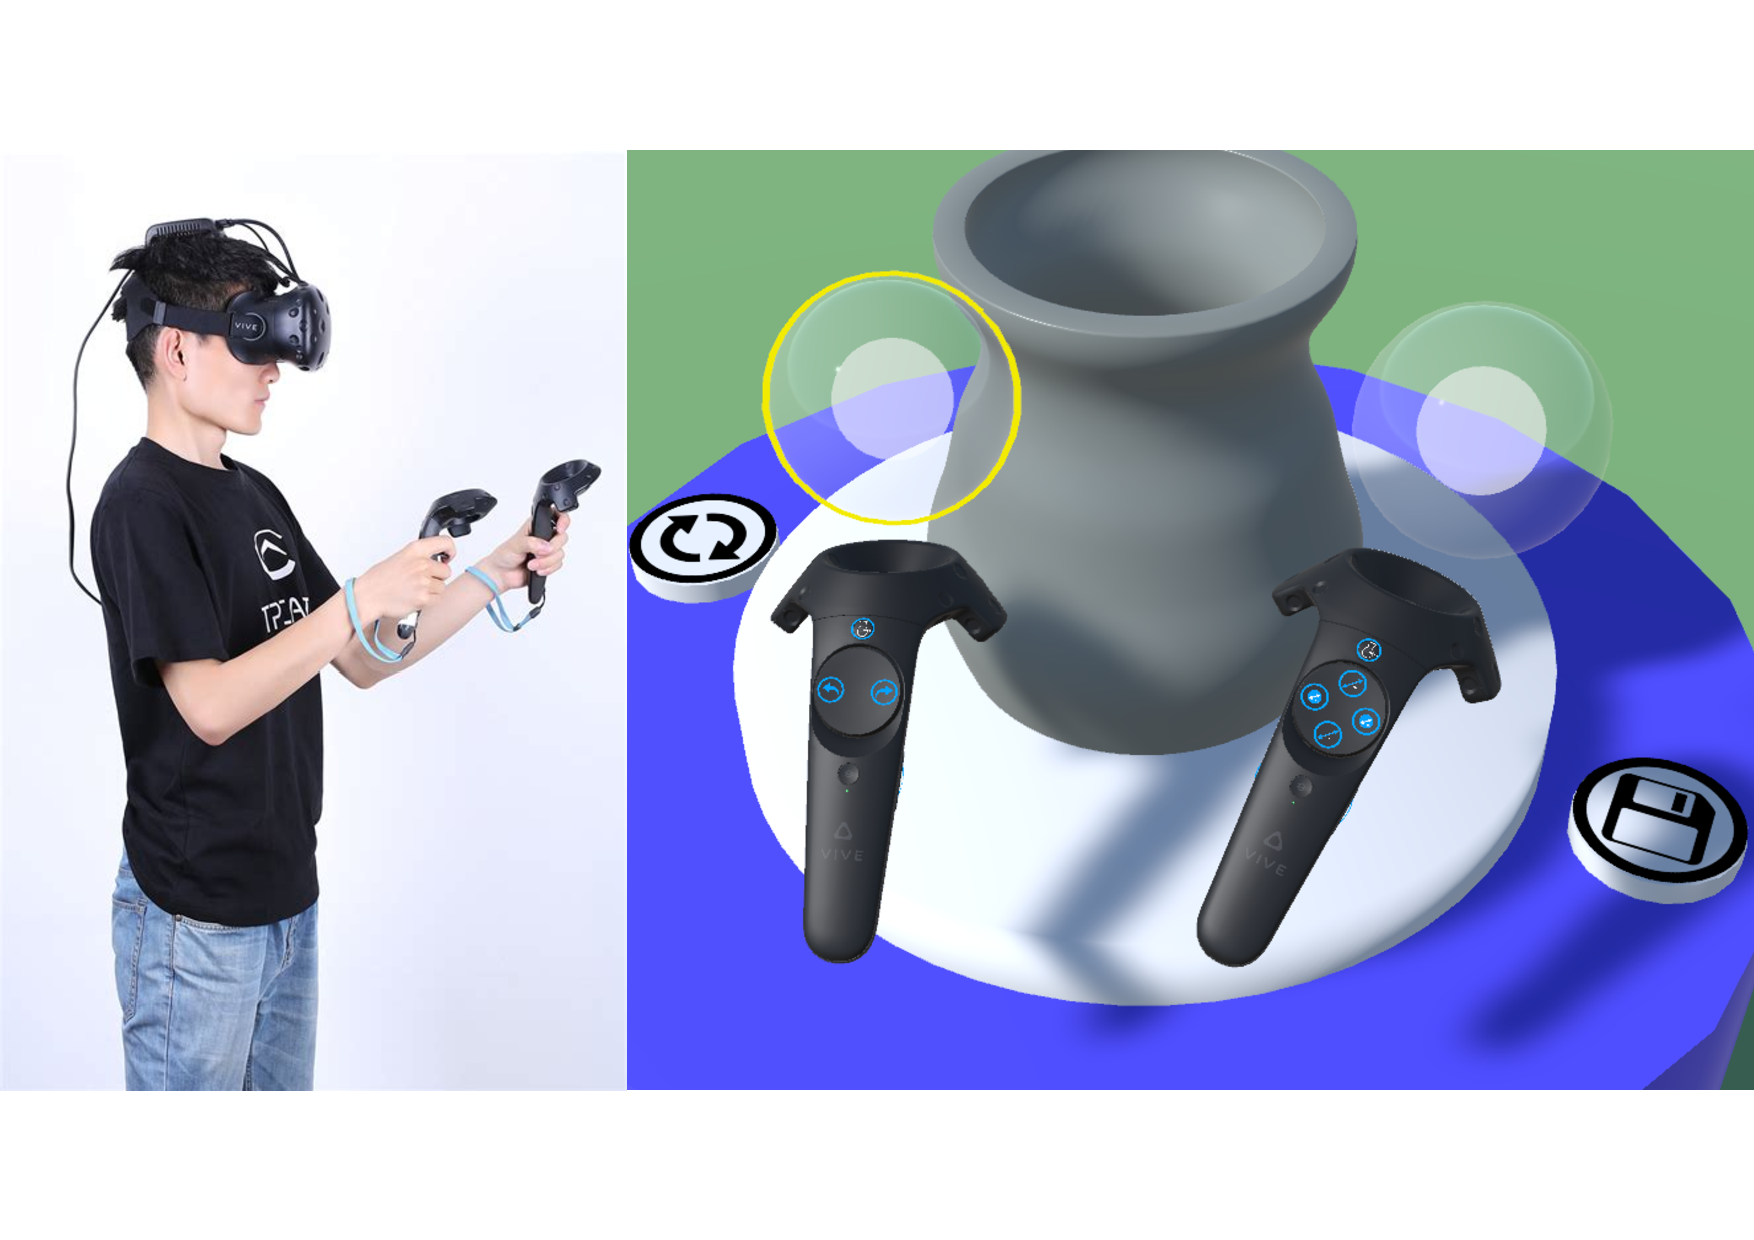
\includegraphics[width=\textwidth]{fig1}
\caption{A user is using our system to create virtual pots.}
\label{fig:demo}
\end{figure}

\subsubsection{System Architecture}
\label{sec:architecture}

The system architecture is demonstrated in Figure \ref{fig:arc}. When the mesh generator generates a clay mesh, users can start to interact with the mesh with handheld haptic devices. The deformation manager is the core component of the mesh editor, which will deform the clay, sending information to haptic manager and UI manager. The haptic manager will send pulses to motion controller as haptic feedbacks, and the UI manager will update the UI elements, sending to the head-mounted display via the rendering engine. Once the creation is done, the mesh IO manager will convert the meshes into OBJ files and save them.

%%%Fig%%% architecture
\begin{figure*}
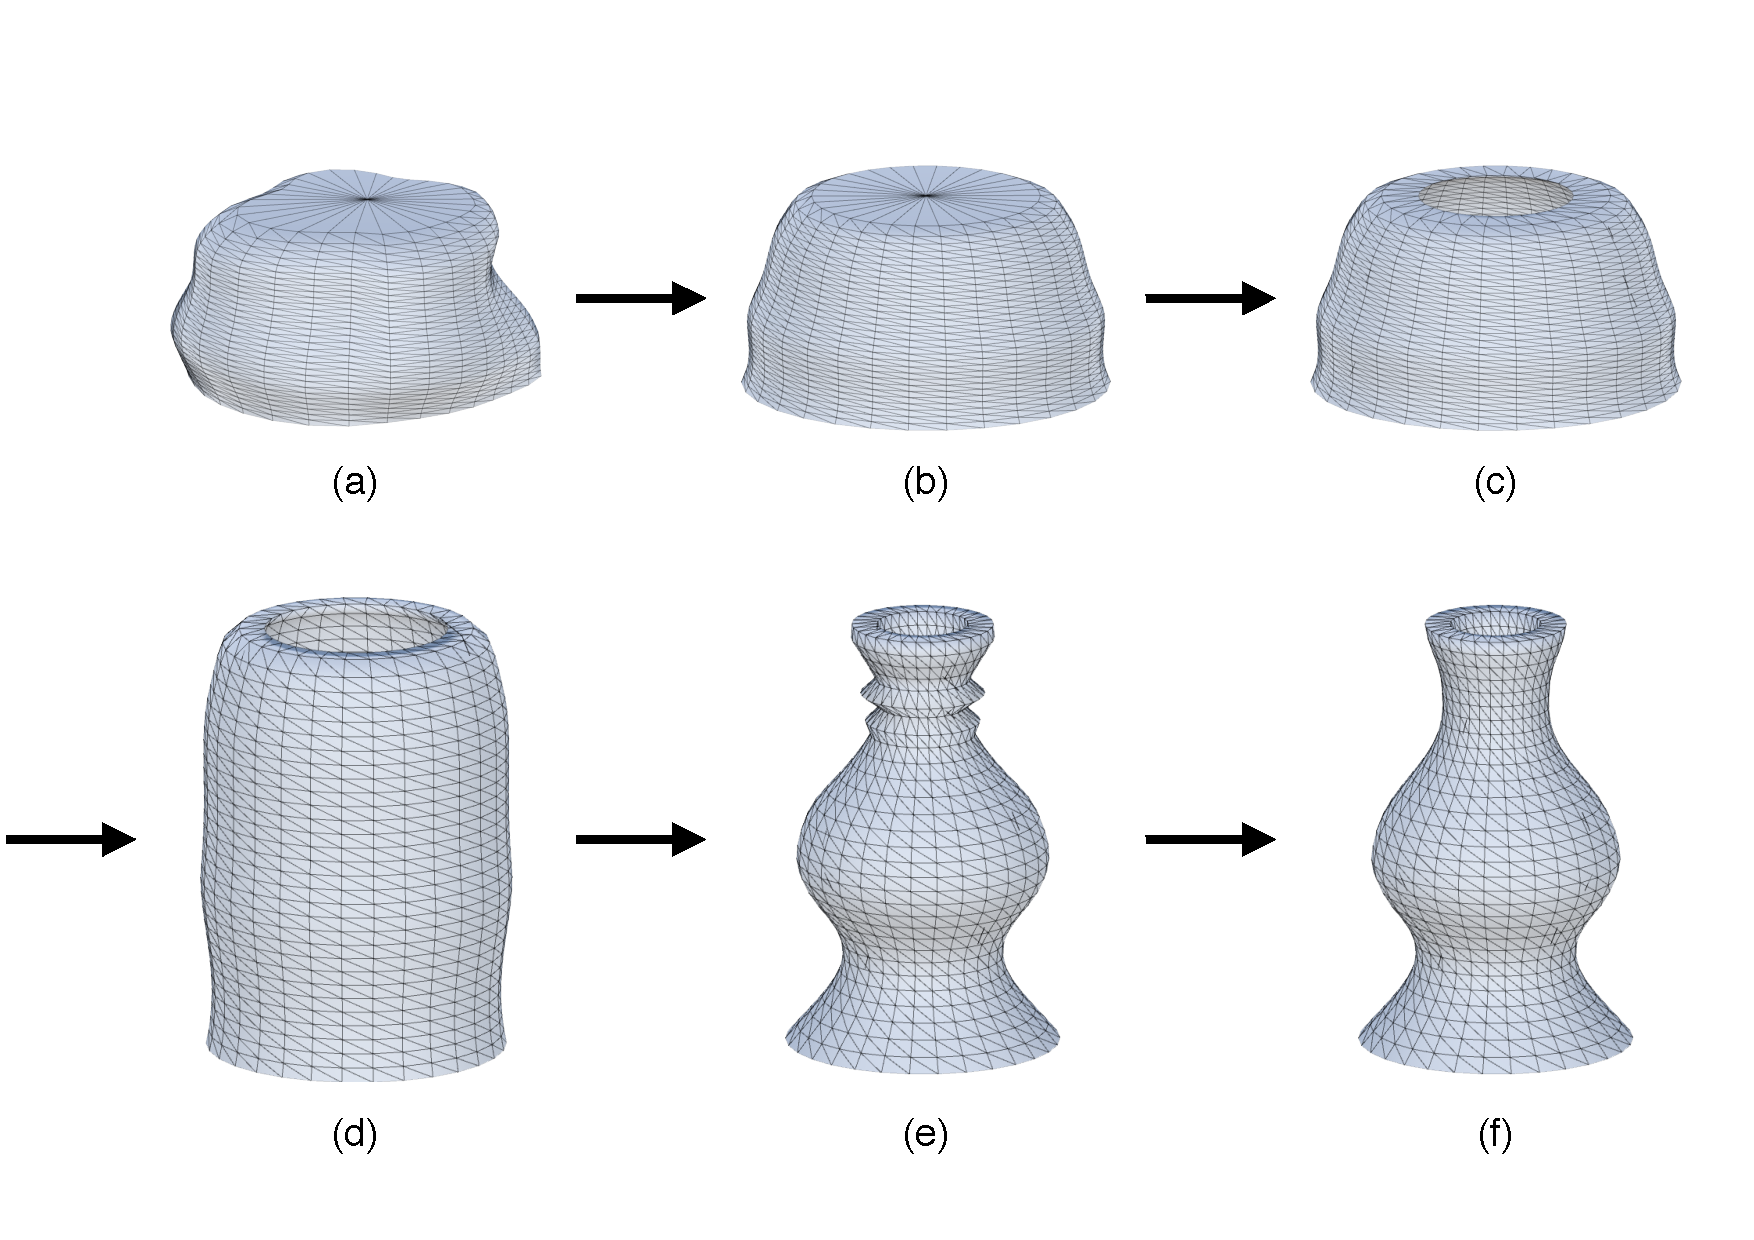
\includegraphics[width=\textwidth]{fig2}
\caption{The system architecture of RealPot.}
\label{fig:arc}
\end{figure*}



\subsubsection{Workflow}
\label{sec:workflow}
In real life, the pottery creation process on a pottery wheel is called \textit{throwing}, where a ball of clay is placed in the center of a turntable wheel-head, and shaped by a potter.
Some interaction metaphors are used in RealPot, which simulates the operations on real-life pottery.
To illustrate the pipeline of pottery creation in our system, an example workflow using RealPot is described as follows.

When a user starts to use RealPot, a realistic clay mesh is automatically generated with Perlin noise (Figure \ref{fig:workflow}a, Section \ref{sec:generation}). 
Similar to the operation in reality, the user first need to use both hands to make the irregular clay shape into perfect rotational symmetry, which is called \textit{centering} (Figure \ref{fig:workflow}b, Section \ref{sec:rotational}).
The user can control the thickness of the clay (i.e. \textit{opening}) by pressing down the clay to create a hollow in the clay (Figure \ref{fig:workflow}c), 
and then draw up the walls with two hands moving up together (i.e. \textit{pulling}), controlling the height of the clay (Figure \ref{fig:workflow}d, Section \ref{sec:thickness}).
The system not only allows mesh deforming (Figure \ref{fig:workflow}e, Section \ref{sec:deformation}) with different deformation range parameters but also mesh smoothing (Figure \ref{fig:workflow}f, Section \ref{sec:smoothing}), where the user can remove sharp features in the pot to get an ideal shape.
After the creation process is finished, the user can export the pottery model as an OBJ file, which can be used for 3D printing.

%%%Fig%%% workflow
\begin{figure*}
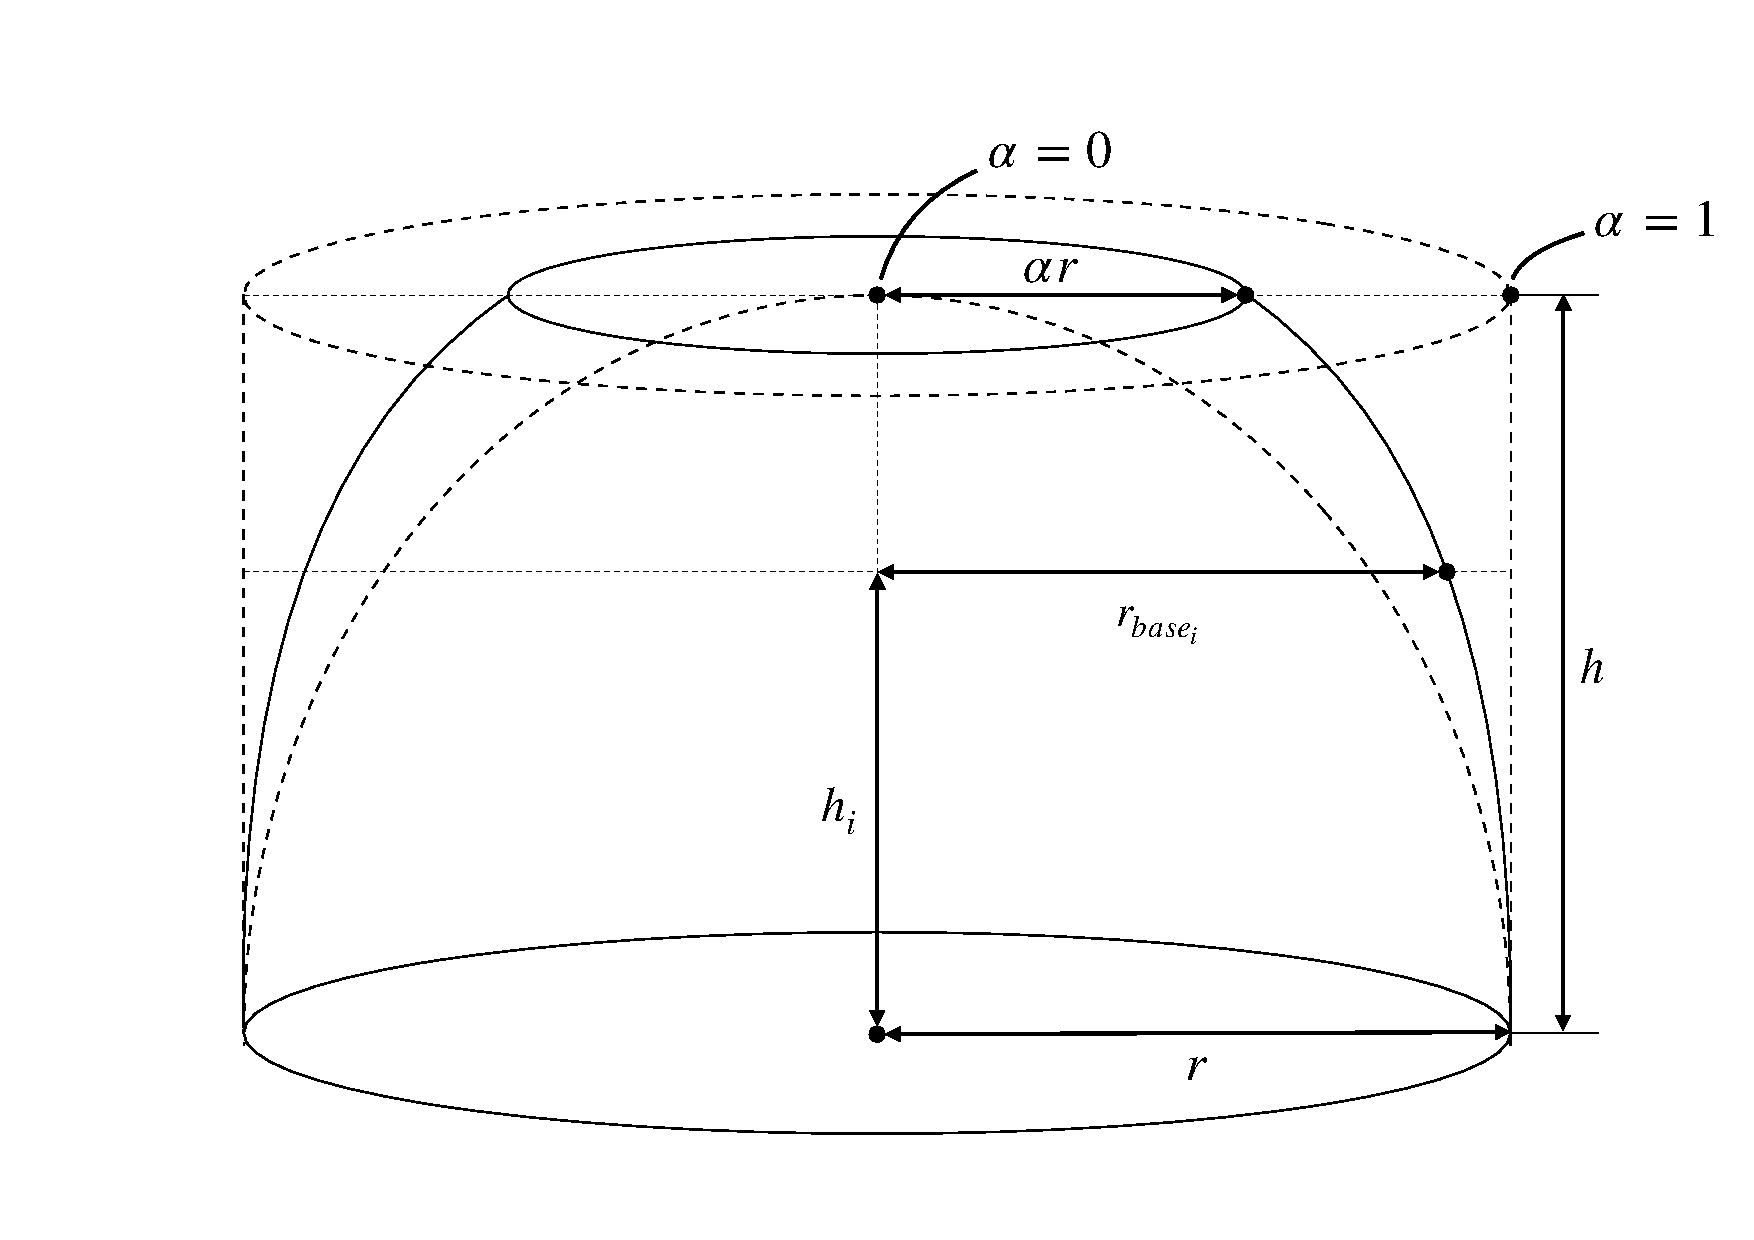
\includegraphics[width=\textwidth]{fig3}
\caption{The workflow in RealPot. (a) The automatically generated clay mesh with Perlin Noise. (b) The mesh is shaped into rotational symmetry by holding both hands. (c) The user controls the thickness of the mesh by pressing down the clay. (d) The user controls the height of the mesh by drawing up the clay wall.(e) The deformation range can be adjusted to get varied deformation effect on different parts. (f) The sharp features on the upper part can be removed by mesh smoothing.}
\label{fig:workflow}
\end{figure*}



\subsection{Mesh Generation}
\label{sec:generation}

Mesh generation is the first step of interactive modeling, and most of virtual pottery systems approximate the initial shape of pottery clay as a primitive cylinder shape \cite{han2007ar,ramani2015gesture,ramani2016extracting}.
Although this approach is simple to implement, it ignores subtle details of clay, whose irregularity needs to be handled first during the creation process in real life.
Unlike the existing virtual pottery systems, RealPot first approximates the initial clay on the pottery wheel as a blending shape of cylinder and semi-ellipsoid, then adds Perlin noises to the basic clay, in order to simulate realistic clay features in reality.

\subsubsection{Basic Clay}

The clay mesh is described as a generalized cylinder, whose resolution can be defined by axis segments $s_{a}$ and height segments $s_{h}$. Given radius $r$ and height $h$, our system can generate primitive mesh of cylinder and semi-ellipsoid respectively (Figure \ref{fig:base}).
For each vertex in the mesh, a $m \times n$ matrix $M$ is used to store radius values, where number of row $m = s_{h} + 1$ and the number of column $n = s_{a}$ respectively. The base radius $r_{base_{i}}$ of each vertex $\mathbf{v}_{i,j}$ in row $i$ can be calculated as: 

\begin{equation}
r_{base_{i}} = \alpha \cdot \frac{r}{h} \sqrt{h^2 -  h_{i}^2} + (1 - \alpha) \cdot r
\end{equation}
\begin{equation}
h_{i} = i \cdot \frac{h}{m-1}
\end{equation}
where $\alpha$ is a factor controls the shape blending between a  cylinder (when $\alpha=0$) and a semi-ellipsoid (when $\alpha=1$) (Figure \ref{fig:base}).

%%%Fig%%% base mesh
\begin{figure*}
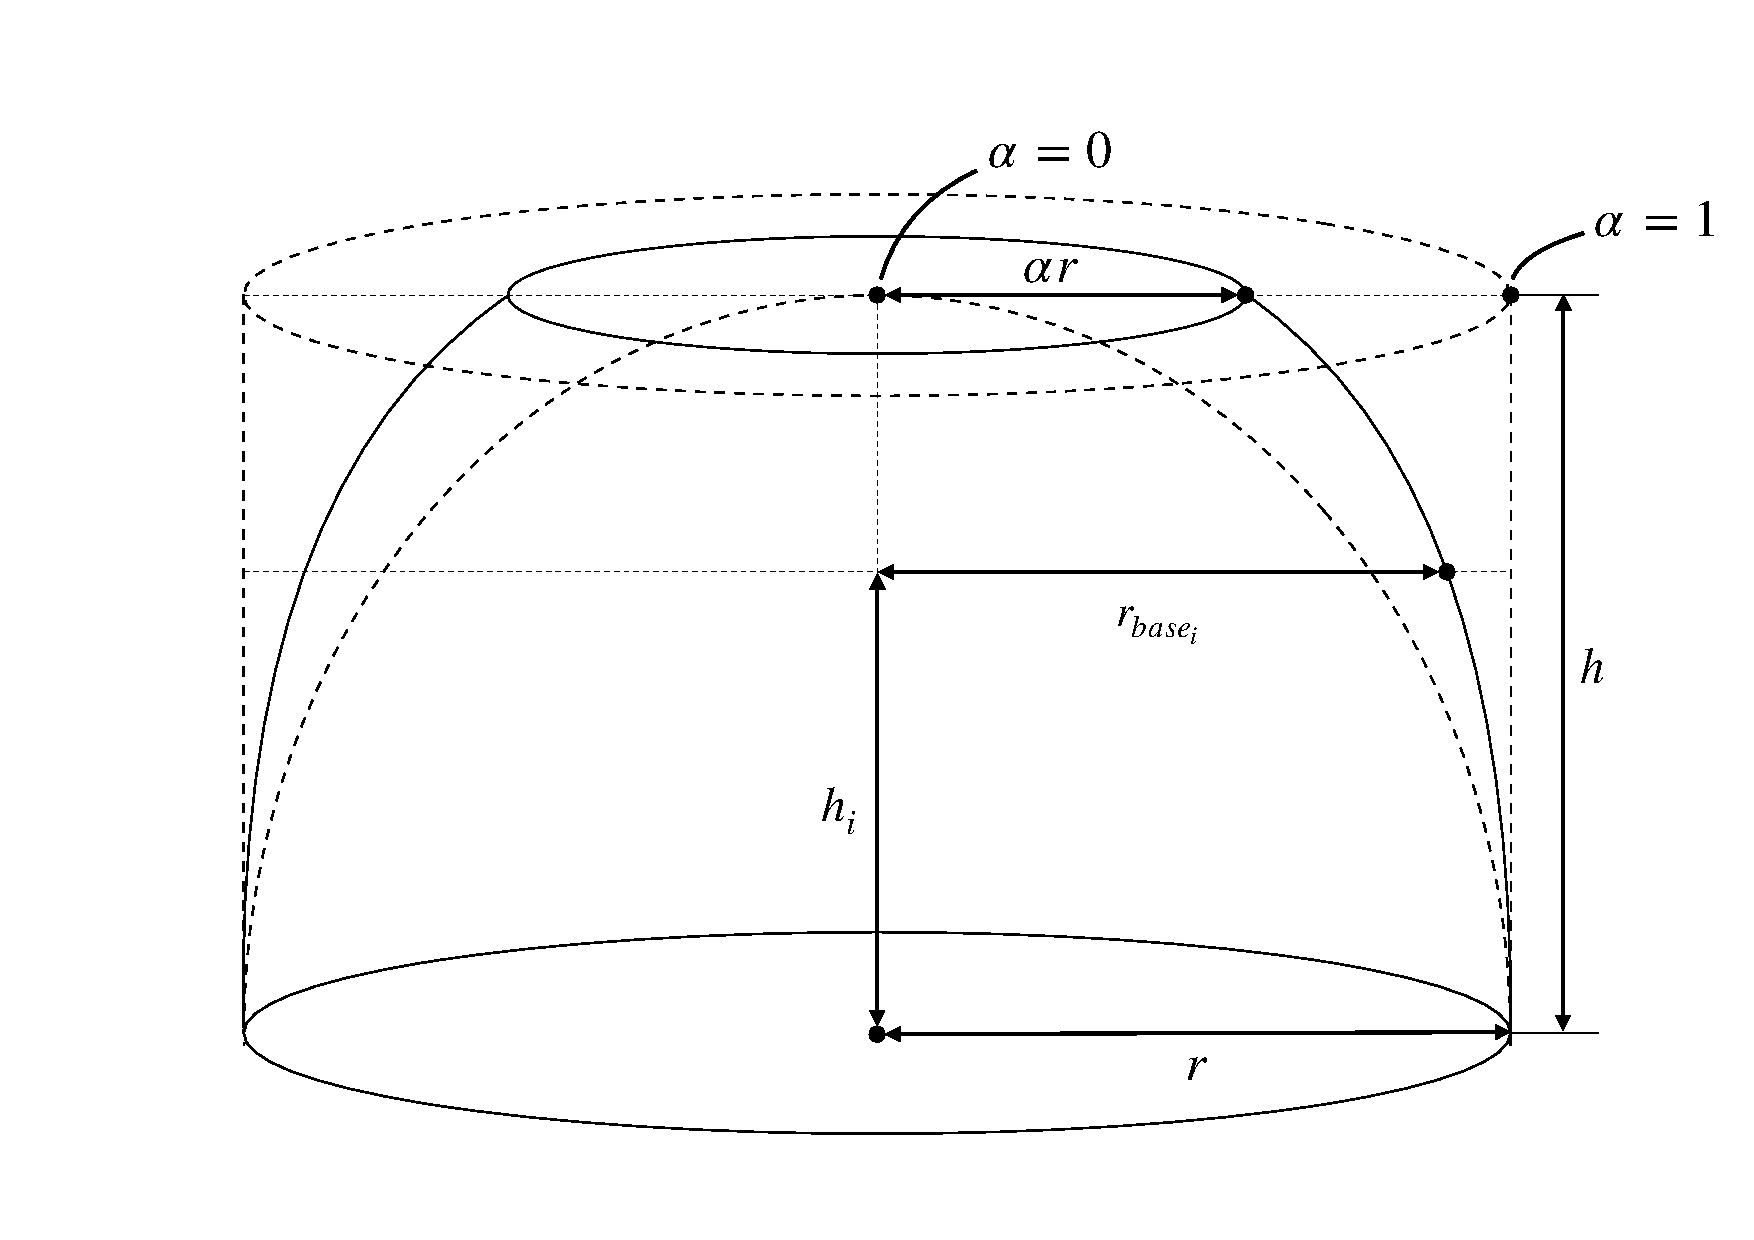
\includegraphics[width=\textwidth]{fig4.pdf}
\caption{The basic clay generated by our system, which is a blending shape between a cylinder and a semi-ellipsoid. $\alpha$ is the blending factor which controls the radius on the top.}
\label{fig:base}
\end{figure*}

\subsubsection{Adding Noise}

Although the initial shape of clay can be roughly approximated like a rotational symmetric shape, in real life, the actual clay shape is not regular, whose irregular features needs to be specially treated during the pottery creation process. To simulate the realistic features, randomness is added to the vertices using Perlin Noise \cite{Perlin1985An}, which is a smooth random method proposed by Ken Perlin in 1985.
In our approach, the center positions for each circular section are randomized first, then Perlin Noise is added to the radii for each circular section and individual vertices.

To add noise to the center for each circular section, random parameters $\phi_{i}$ and $\eta_{c_{i}}$ are used to calculate the new center $\mathbf{O}_{i}$:
\begin{equation}
\label{eqn:oi}
\mathbf{O}_{i} = \left[\eta_{c_{i}}cos\phi_{i}, h_{i}, \eta_{c_{i}}sin\phi_{i}\right]^T
\end{equation}
where $\phi_{i} \in [0, 2\pi]$ is a random degree, and $\eta_{c_{i}}$ is a random radius.
Then the new radii $r_{total_{i,j}}$ for each vertex can be computed by getting the sum of $r_{base_{i}}$ and noise values:
\begin{equation}
r_{total_{i,j}} = r_{base_{i}} + \eta_{row_{i}} + \eta_{indv_{i,j}}
\end{equation}
where $\eta_{row_{i}}$ is the radius noise for each circular section, and $\eta_{indv_{i,j}}$ is the individual radius for each vertex (Figure \ref{fig:noise}). The radius value $r_{i,j}$, along with the position $\mathbf{v}_{i,j}$ for each vertex can be computed in the follow equations:
\begin{equation}
r_{i,j} = \left\|
\mathbf{O}_{i} + \left[ r_{total_{i,j}} cos \theta_{j},
0,
r_{total_{i,j}} sin \theta_{j}
\right]^T
\right\| 
\end{equation}

\begin{equation}
\theta_{j} = j \cdot \frac{2\pi}{n}
\end{equation}

\begin{equation}
\label{eqn:v}
\mathbf{v}_{i,j} =
\left[r_{i,j}  cos \theta_{j},
h_{i},
r_{i,j} sin \theta_{j}\right]^T
\end{equation}

%%%Fig%%%
\begin{figure*}
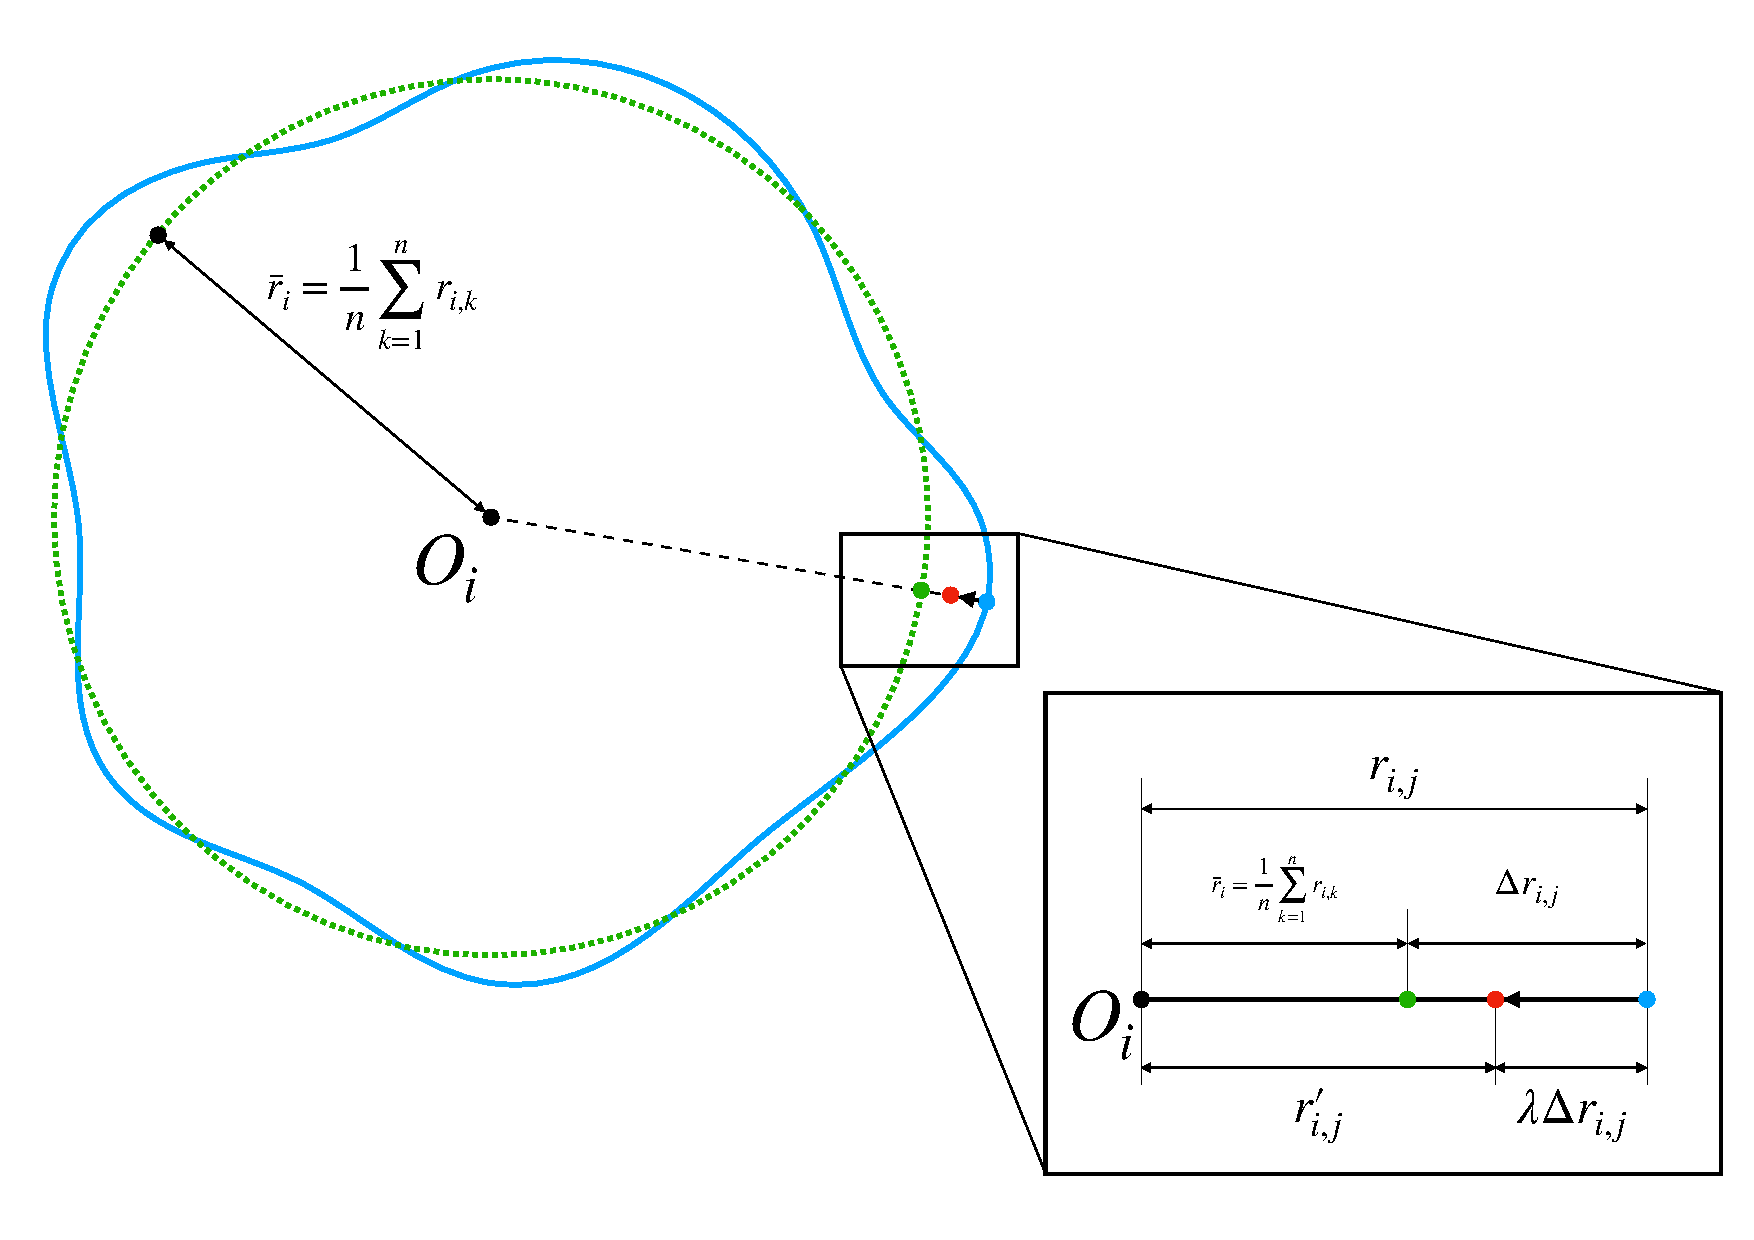
\includegraphics[width=\textwidth]{fig5.pdf}
\caption{To get a noised radius $r_{i,j}$ (green) based on radius $r_{base_{i}}$ (red): (1) Move the center from origin (0,0) to $\mathbf{O}_{i}$. (2)Calculate the sum: $r_{total_{i,j}} = r_{base_{i}} + r_{row_{i}} + r_{indv_{i,j}}$. (3) Find the distance to the origin, which will be the noised radius $r_{i,j}$.}
\label{fig:noise}
\end{figure*}

\subsubsection{Inner Vertices}

To create 3D printing oriented pottery models, our system needs to generate watertight 3D models with thickness.
To accomplish that, RealPot generates inner and bottom sides based on the outer side mesh. The vertices on inner side can be denoted as:

\begin{equation}
\label{eqn:v'}
\mathbf{v'}_{i,j} 
= \begin{cases}
\begin{bmatrix}
0,h_{i},0
\end{bmatrix}^T & \beta=1
\\
\begin{bmatrix}
r'_{i,j} \cdot cos \theta_{j},
h_{i},
r'_{i,j} \cdot sin \theta_{j}
\end{bmatrix}^T & 0 \le \beta<1
\end{cases}
\end{equation}

\begin{equation}
r'_{i,j} = r_{i,j} - \max(t_{min}, r_{top} \cdot \beta)
\end{equation}
where $\beta$ is the thickness ratio of the clay, whose range is $[0,1]$. In mesh generation phase, the default value of $t$ is 1, which means the clay is a solid shape; in mesh deformation phase, the value of $t$ can be adjusted by users interactively, getting a center-hollowed shape. $t_{min}$ is a predefined value for the minimum thickness, and $r_{top}$ is the largest radius value for the top section, which guarantees equal thickness for each part.
Vertices for inner-bottom and outer-bottom sides will be then generated according to inner-side and outer-side vertices respectively. Finally, a mesh can be generated by constructing triangle faces based on the vertex indices (Figure \ref{fig:mesh}).

%%%Fig%%% Mesh
\begin{figure}
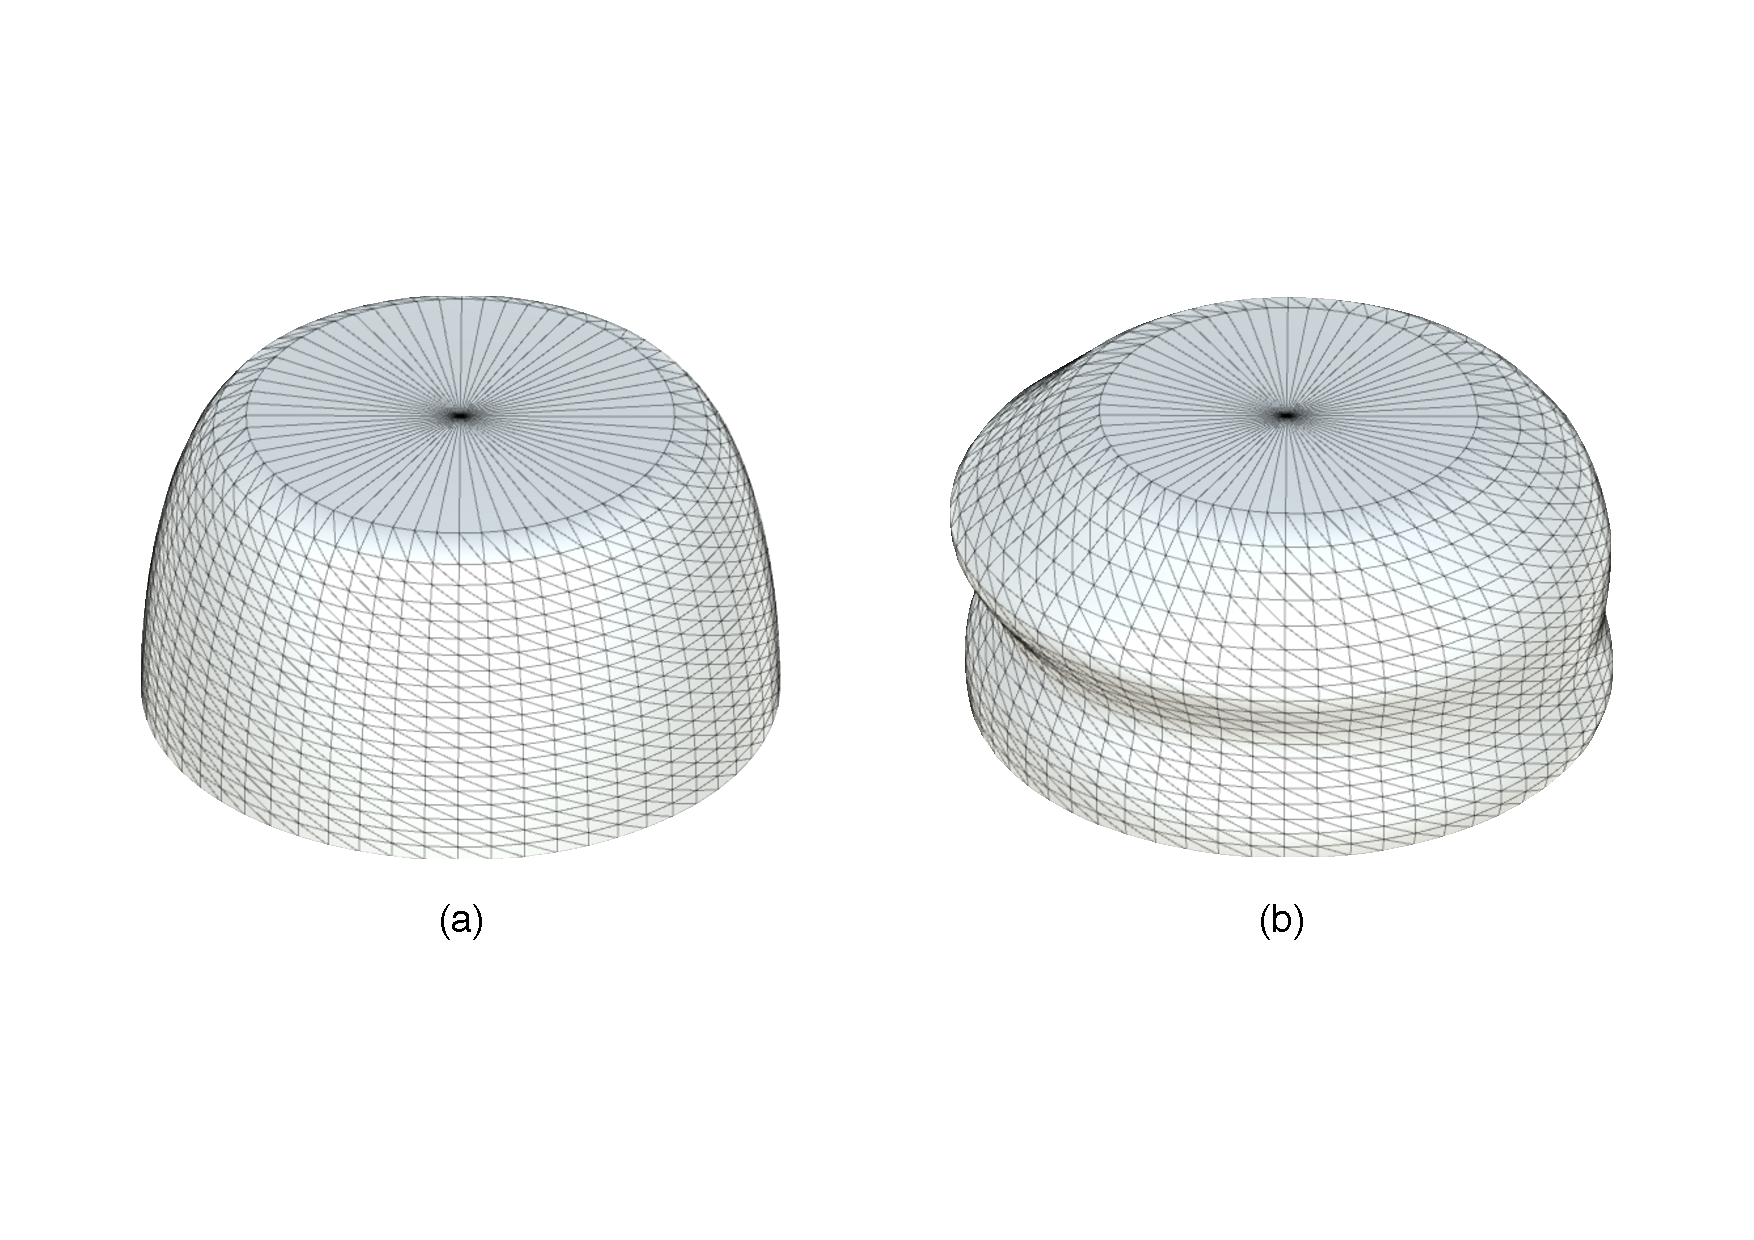
\includegraphics[width=\textwidth]{fig6}
\caption{The meshes generated with our system. (a) A regular mesh without adding Perlin noise. (b) A mesh with Perlin noise, which is more realistic as a clay.}
\label{fig:mesh}
\end{figure}

\subsection{Mesh Editing}
\label{sec:editing}
After observing and analyzing several real-life pottery throwing videos, we put real-life clay operations into 5 categories: (1) rotational symmetry control, (2) thickness control, (3) height control, (4) mesh deformation and (5) mesh smoothing.
And we propose 5 interaction metaphors in our system: \textit{centering}, \textit{opening}, \textit{pulling}, \textit{shaping} and \textit{smoothing}, which correspond to the clay operations above.
These operations will be discussed in detail in the following sections.
Since any clay mesh $C$ can be generated from key parameters including height $h$, thickness $t$ and radius matrix $M$, a mesh generation function is constructed: $C =  g(h, t, M)$, which can be used to update the mesh data as well.
In our approach, RealPot first modifies key parameters of the clay according to user interactions, then updates mesh data $C$ in realtime based on these parameters using the mesh generation function.

\subsubsection{Rotational Symmetry Control}
\label{sec:rotational}
\textit{Centering} is the first important operation in pottery creation in reality, where people press the ball of clay downward and inward, making the irregular clay into perfect rotational symmetry.
In our system, the user can use two controllers to touch the virtual clay and pull the trigger button to achieve symmetry control (Figure \ref{fig:workflow}b).
The mean radius value of each row in the radius matrix is calculated and then each radius value in matrix needs updating based on the mean radius values:
\begin{equation}
\label{eqn:sym}
r'_{i,j} = 
\lambda \cdot \frac{1}{n}\sum_{k=1}^{n} r_{i,k}
+ (1 - \lambda) \cdot r_{i,j}
\end{equation}
where $\lambda \in [0,1]$ is a damping factor controlling the rate of symmetry.
The effect of rotational symmetry control is illustrated in Figure \ref{fig:symmetry}.

%		Fig:Symmetry
\begin{figure*}
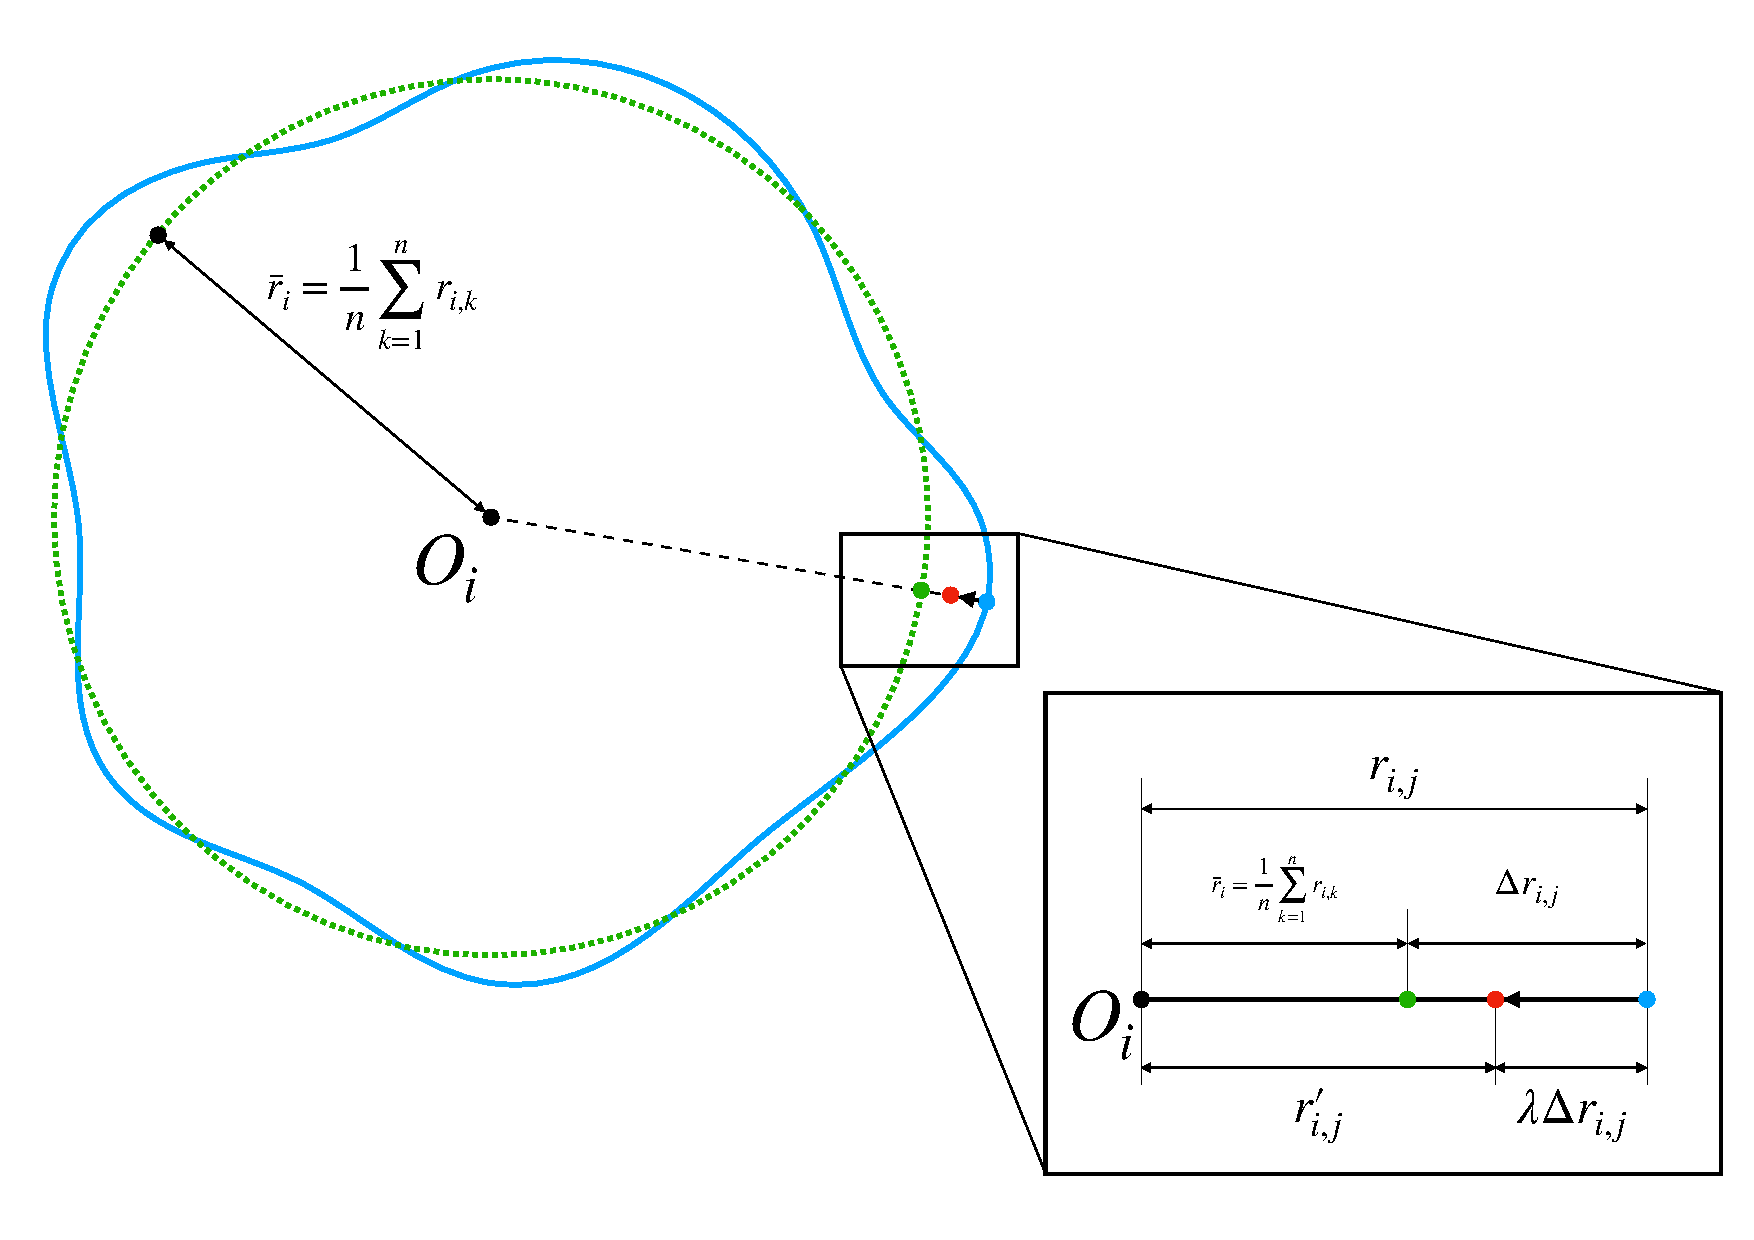
\includegraphics[width=\textwidth]{fig7.pdf}
\caption{Rotational symmetry control. The blue curve is the noised circular section at height $h_{i}$, and the green curve is a circle with the average radius $\bar r_{i}$. Let $\Delta r_{i,j}$ be the difference between $r_{i,j}$ and $\bar r_{i}$, then multiplied by the damping factor $\lambda$. New radius be calculated : $r'_{i, j} = r_{i,j} - \lambda\Delta r_{i}$, which is identical to Equation (\ref{eqn:sym}). }
\label{fig:symmetry}
\end{figure*}

\subsubsection{Thickness and Height Control}
\label{sec:thickness}
\textit{Opening} (thickness control) and \textit{pulling} (height control) are basic clay operations in pottery throwing process which are done by applying force to clay with both hands. The thickness can be adjusted by pushing down the top center part of the clay, making a centered hollow into the clay (Figure \ref{fig:workflow}c). The height can be adjusted by both hands drawing up and shaping the walls (Figure \ref{fig:workflow}d).
Let $\Delta y$ be the mean of $\Delta y_{l}$ and $\Delta y_{r}$, which are left and right vertical hand movement distance respectively. New height $h'$ and new thickness ratio $\beta'$ can be calculated in the following equations:
\begin{equation}
\Delta y = (\Delta y_{l} + \Delta y_{r})/2
\end{equation}
\begin{equation}
h' = h_{0} + \Delta y * \gamma
\end{equation}
\begin{equation}
\beta' = \beta_{0} + \Delta y/ h
\end{equation}
where $h_{0}$ and $\beta_{0}$ are initial height and thickness ratio values before deformation respectively; $\gamma$ is a damping factor for height. And the new mesh data will be recomputed using new values $h'$ and $\beta'$.

\subsubsection{Mesh Deformation}
\label{sec:deformation}
In this section, interactive deformation in our system will be discussed. According to \cite{botsch2010polygon}, this topic is challenging since complex mathematical formulations (1) have to be hidden behind an intuitive user interface and (2) have to be implemented in a sufficiently efficient and robust manner to allow for interactive applications.

In our approach, a cylindrical coordinate system is used to specify the position for each vertex, where y-axis is the reference axis. For any point $P$ in the coordinate system, we use$(\rho, \phi, y)$ to denote the position, where the radial distance $\rho$ is the Euclidean distance from the y-axis to the point P; $\phi$ is the azimuth; $y$ is the height of point P from xz-plane.
Due to rotational symmetry in virtual pottery, RealPot modifies the $\rho$ for each vertex while keeping $\phi$ and $y$ constant. Thus, the deformation problem is turned into how to calculate the new radius $\rho'_{i,j}$ based on hand movement:
\begin{equation}
\rho'_{i,j} = \rho_{i,j} + \Delta \rho_{i,j}
\end{equation}

% base on 3D cursor radial dist
Let $(x_{0},y_{0},z_{0})$ be the initial 3D cursor position at time $t_{0}$ when the deformation starts, and we can calculate the initial radial distance of the 3D cursor from y-axis: $\rho_{0} = \sqrt{x_{0}^2 + z_{0}^2}$. The new 3D cursor position at time $t_{1}$ is $(x_{1},y_{1},z_{1})$, and the new radial distance is $\rho_{t} = \sqrt{x_{1}^2 + z_{1}^2}$.
% vertical dist
When the user presses the trigger button on the controller while the 3D cursor touches the mesh, the vertical distance $d_{i,j}$ between the 3D cursor and each vertex $\mathbf{v}_{i,j}$ can be computed as:
\begin{equation}
d_{i,j} = |y_{0} - y_{i,j}|
\end{equation}
where $y_{i,j}$ is the height of $\mathbf{v}_{i,j}$.
In our system, outer range $R_{O}$ and inner range $R_{I}$ are two key parameters affecting deformation effect, which divides the mesh into three regions: fixed region, moving region and  deformation region (Figure \ref{fig:deform}a).
The fixed region will keep constant during the deformation, where $d_{i,j} > R_{O}$; the moving region will follow the movement of the 3D cursor, where $d_{i,j} < R_{I}$; and the deformation region will be affected based on the weights, where $R_{I} < d_{i,j} < R_{O}$.
%The deformation region should deform in an intuitive and smooth manner.
Note that when $R_{I} = 0$, the deformation will go in a smooth way; when $R_{I} = R_{O}$, it is possible to create sharp features on the clay:
\begin{equation}
\Delta r_{i,j} = \begin{cases}
\rho_{t} - \rho_{0} &  d_{i,j} < R_{I} \\
0 &  d_{i,j} > R_{O} \\
(\rho_{t} - \rho_{0}) \cdot w_{i,j} &  R_{I} < d_{i,j} < R_{O}
\end{cases}
\end{equation}

%get weight from falloff curve
A falloff curve is needed in order to get smooth deformation effect when calculating weights: $w_{i,j} = f(t)$, where $t = (d_{i,j} - R_{I}) / (R_{O} - R_{I})$.
There are many ways to select a smooth falloff functions for the weights, which needs to satisfy these additional requirements: (i) f(0) = 1 , (ii) f(1) = 0 and (iii) f'(0) = f'(1) = 0.
In order to efficiently calculate the weights, we choose a cubic polynomial function $f(t) = at^3 + bt^2 + ct + d$ as the weight falloff function, we have:
\begin{equation}
\begin{aligned}
\label{equation:falloff}
f(0) = 1 \\
f(1) = 0 \\ 
f'(0) = 0 \\
f'(1) = 0
\end{aligned}
\end{equation}
we can find the solution from Equation (\ref{equation:falloff}), where 
$a = 2, b = -3, c = 0, d = 1$. Therefore, the expression of the falloff function is $f(t) = 2t^3 - 3t^2 + 1$ (Figure \ref{fig:deform}b).

%%%Fig%%%
\begin{figure*}
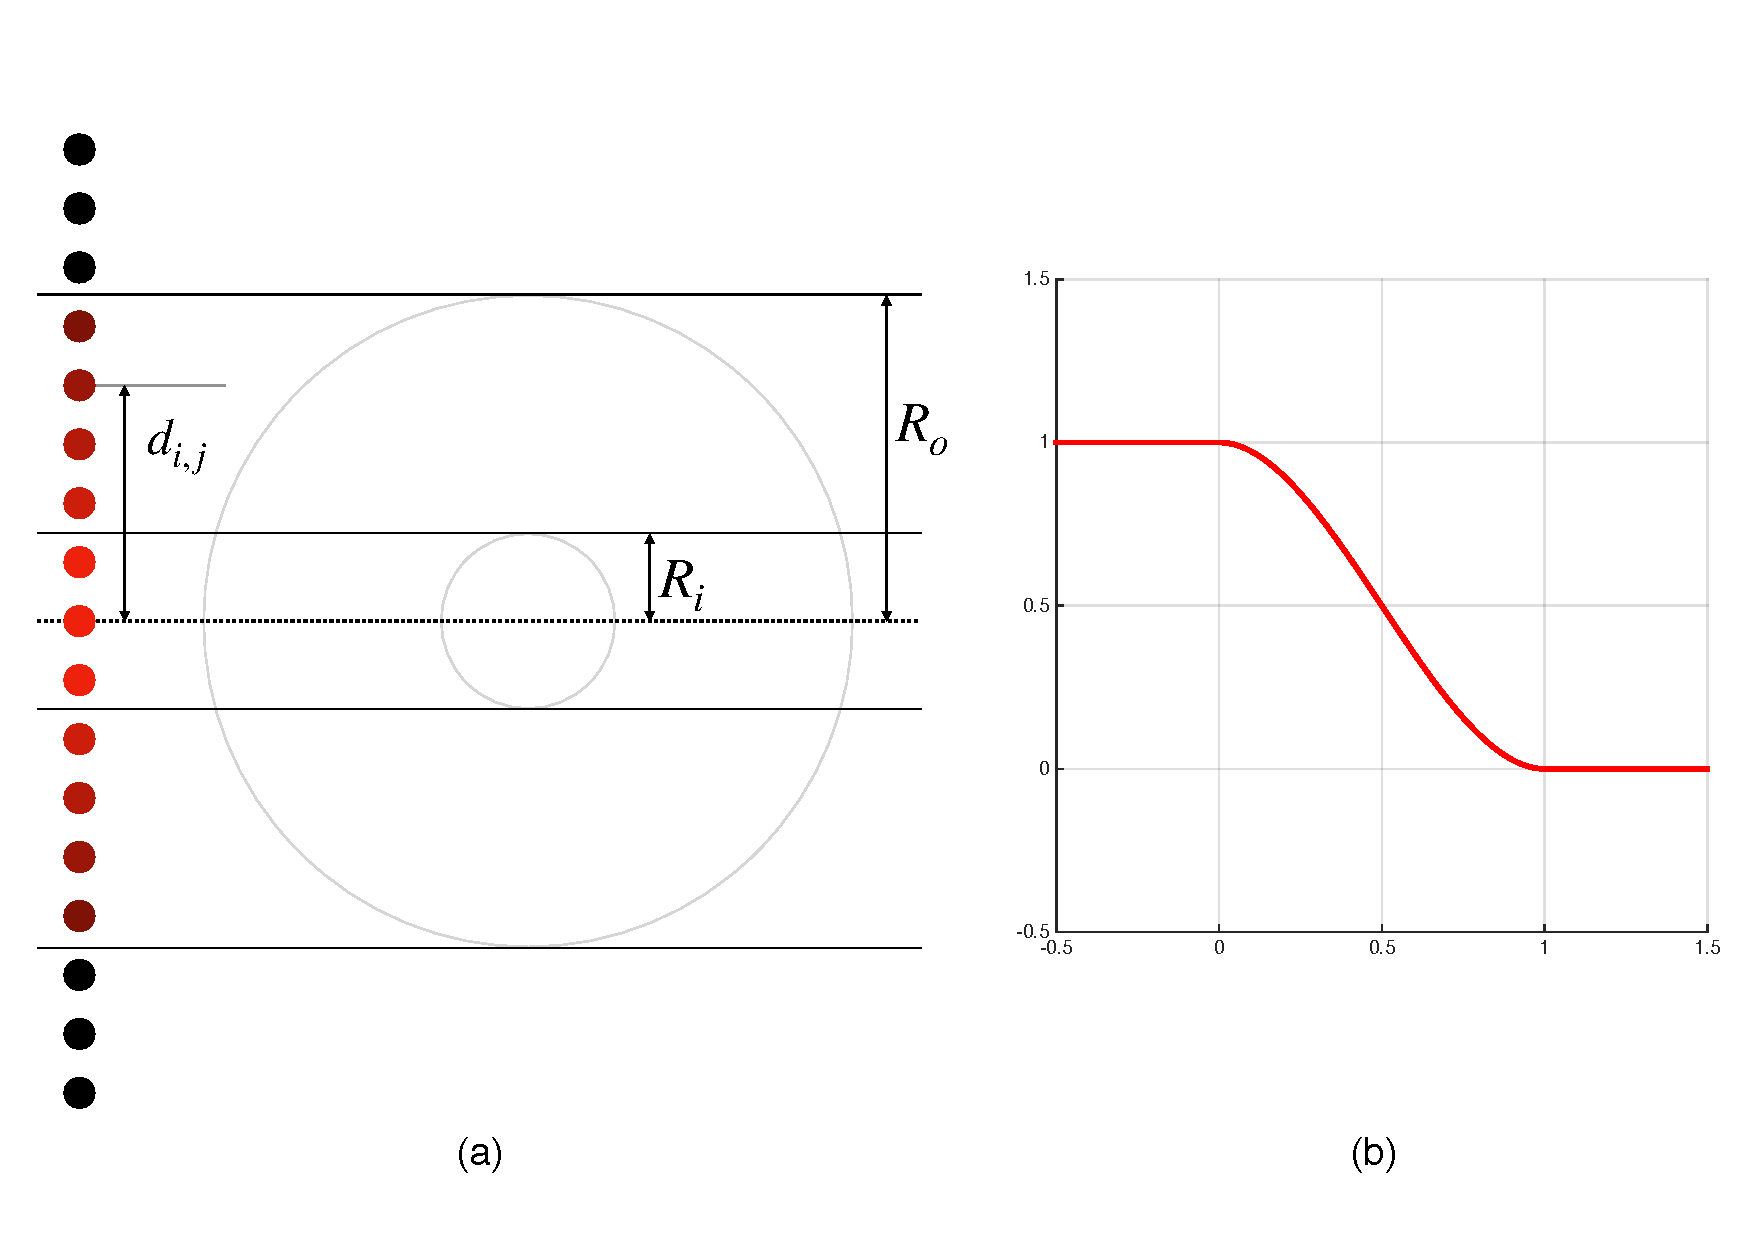
\includegraphics[width=\textwidth]{fig8.pdf}
\caption{(a) The concentric circles represent the 3D cursor, and $R_{I}$ and $R_{O}$ define the inner range and outer range respectively. $d_{i,j}$ is the vertical distance between a vertex $\mathbf{v}_{i,j}$ in the deformation region and the 3D cursor, which is used for calculating weight parameter : $t = (d_{i,j} - R_{I}) / (R_{O} - R_{I})$. (b) A cubic polynomial function $f(t) = 2t^3 - 3t^2 + 1, t \in [0,1]$ is used as the falloff curve for calculating the weight $w_{i,j}$. }
\label{fig:deform}
\end{figure*}

\subsubsection{Mesh Smoothing}
\label{sec:smoothing}
As mentioned above, it is possible to create sharp features upon the clay mesh during the deformation process. In order to remove unwanted sharp features, our system uses Laplacian smoothing:
\begin{equation}
r'_{i,j} = 
\omega  \frac{1}{N} 
\sum_{k=1}^N r_{k}
+ (1 - \omega)  r_{i,j}
\end{equation}
where $N$ is the number of adjacent vertices of $\mathbf{v}_{i,j}$; $\omega \in [0,1]$ is a factor controlling the smoothing effect.
Only the vertices within the range of the 3D cursor $R_{O}$ will be affected.
As a result, users can control the 3D cursor position and adjust the outer range $R_{O}$ of the 3D cursor to apply smoothing on specific areas interactively on the mesh.

%%% HAPTIC
\subsection{Haptic Feedback Model}

Haptic feedbacks can be crucial when touching or grasping an object in virtual environments, which are helpful for users to perceive the location of virtual objects.
However, little work has been done on haptic feedbacks in the existing virtual pottery systems, due to their intrinsic barehand-based interaction mechanisms.
To increase the fidelity of our system, a haptic feedback model for virtual pottery is described  in this subsection.
Unlike the barehand experience, RealPot provide users with rich haptic feedbacks by handheld controllers based on the proposed model.

%Unlike the barehand experience, instrument-based interactions can provide haptic feedbacks, adding realistic feel in VR environments. In our system, a haptic pulse has been added to a controller when that controller has touched the clay. During any mesh editing process, we add movement resistance feedback based on the movement speed of each hand.


\subsubsection{Analysis of the sensation in pottery}

In real life pottery, users can perceive forces from hands and fingers when performing various operations on the clay.
In addition, users can obtain information from these forces, such as shape and smoothness etc.

To provide realistic haptic feedbacks in our system, we analyzed the pottery throwing process in real life.
In general, the haptic feedbacks from clay can be classified into two categories based on the type of forces: friction force and reaction force.
When a user softly touches the clay without pushing or pulling, he/she can perceive the sensation on fingers or hands since the clay is rotating.
Moreover, when a user pushes or pulls to deform the clay, reaction forces are generated in the opposite direction to the movement.

% in our system, ? are provided to the user.

From the analysis, clay various changes including...(i)friction (ii)reaction

As described in Section \ref{sec:editing}, there are five main mesh editing operations in our system.

% ??? Among the five operations, both friction force and reaction force will be generated.

By designing mechanisms that simulate the forces, we can realize a virtual pottery system with realistic haptic feedbacks.
The mechanisms will be described in detail in the following subsections.

%5// friction from rotation

%// factors - pressure and dryness, smoothness

%6// reaction force

%// depends on the force, hand acceleration

\subsubsection{Friction Haptic Model}

%The direction of the force is ...

%The magnitude of the force is ...

%The friction force is the pressure.

% changes according to the amount of pressure applied to the clay.

%// The hand will get frictional force when touching the rotating clay
%// can will get extra force when trying to centering or smoothing by applying pressure


%//When the hand start to contact with the rotating clay, the user can perceive the sensation of touching the clay surface. The roughness of the contact surface and the pressure 

In this subsection, we describe a model to calculate the friction force, which is generated when the user touches the surface of the rotating clay.

For calculation efficiency, we assumed the friction type as kinetic friction, which is a force that opposes the relative motion between moving surfaces.
The frictional force can be calculated by the following equation:

\begin{equation}
F_{f} = \mu \cdot F_{n}
\end{equation}

where $\mu$ is the coefficient of friction between clay and hand, and $F_{n}$ is the normal force exerted on the clay surface.

Since all the mesh editing operations in our system can be performed using handheld controllers, we use the trigger value as the input of normal force.

The trigger value ranges from 0 to 1, which indicates how much has the user pulled the trigger button.

% when the trigger is not pressed and the controller is contacted with the clay. -> minimum friction

In the HTC VIVE handheld controllers, haptic feedback is generated by the built-in vibrators.
The haptic pulse intensity based on friction is calculated as:

\begin{equation}
k_{f} = k_{min} + \epsilon \cdot k_{\mu}
\end{equation}
where $k_{0}$ is the minimum friction intensity when user just touches the clay, and $\epsilon \in [0,1]$ is analog value of the trigger button. $k_{\mu}$ is the predefined coefficient.


\subsubsection{Reaction Haptic Model}

In actual pottery creation processes, users often exert forces to deform the clay by pushing or pulling.

According to Newton's Third Law, the forces between the hand and the clay exist in equal magnitude and opposite direction.

Since handheld controllers are used in our system, the reaction force exerted by hands can be calculated based on the position of the controllers.

\begin{equation}
\mathbf{F} = m \frac{\mathrm{d} \mathbf{v}}{\mathrm{d} t}
\end{equation}
Since both the hand mass $m$ and frame time interval $\Delta t$ are constant, a predefined value $k_{\omega}$ is used in the follow equation to calculate 


The reaction haptic intensity $k_{r}$ in each frame can be calculated based on the consecutive controller positions in last three frames:

\begin{equation}
k_{r} = k_{\nu} \cdot \|\mathbf{v} - \mathbf{v}'\| = k_{\nu} \cdot \|(\mathbf{x}-\mathbf{x}') - (\mathbf{x}'-\mathbf{x}'')\| = k_{\nu} \cdot \|\mathbf{x}-2\mathbf{x}'+\mathbf{x}''\|
\end{equation}

Here, $k_{\nu}$ is a predefined coefficient; $\mathbf{x}$ is the controller position in current frame; $\mathbf{x}'$ and $\mathbf{x}''$ are the consecutive controller positions in last two frames.

The total hapic intensity is the sum of friction force and reaction force.

\begin{equation}
k_{\sigma} = k_{r} + k_{f}
\end{equation}

From the above, the user can perceive rich haptic feedback when shaping the virtual pottery.

By providing haptic feedback based on $k_{\sigma}$, we can implement the sensation caused by clay deformation.

%the reaction force is opposite to the force exerted on the clay

%We can consider clay apply reaction force to the hands when we apply force to the clay.

%According to Newton's Third Law, the reaction force $F_{r}$ from the clay is opposite to the force $F_{h}$ exerted by hand. 
%According to Newton's second law, the reaction force can be calculated as follows:



%In addition, visual feedback
In a VE, it is not so easy for users to perceive if her hands have touched anything. Hence, our system adds visual feedback on both virtual sphere, which will be highlighted when touching the clay (Figure \ref{fig:highlight}).


%%%Fig%%% Highlight
\begin{figure}
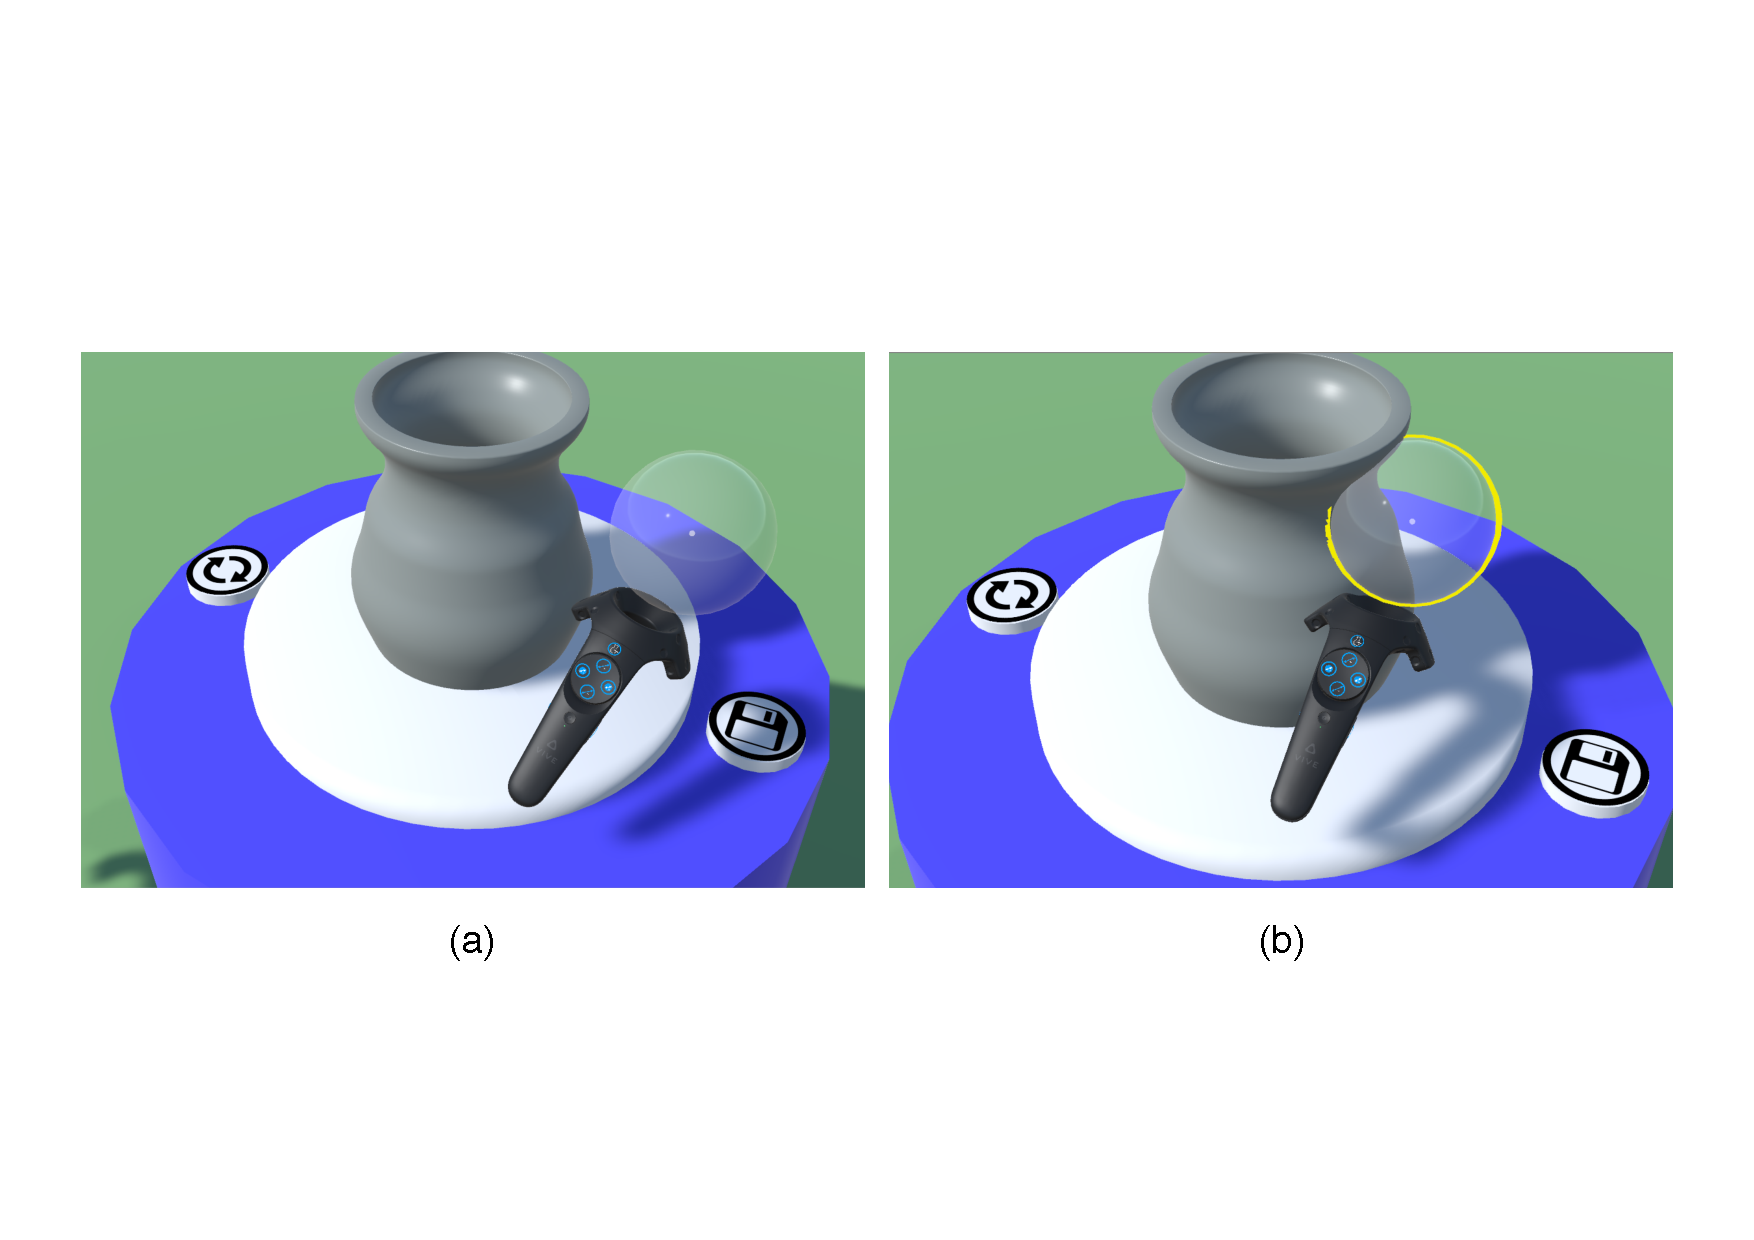
\includegraphics[width=\textwidth]{fig10}
\caption{The visual and haptic feedback when user touches the clay. (a) The normal state of the 3D cursor when it is not touching the clay. (b) The highlight state of the 3D cursor when a user has touched the clay, with a haptic pulse to the corresponding hand.}
\label{fig:highlight}
\end{figure}

%%%


\subsection{Interactions}
\label{sec:interactions}

%%%Fig%%% UI


%the system in a virtual studio - pottery wheel
RealPot is designed as a pottery studio built in a VE.
In our implementation, we use a HTC Vive VR system \cite{website:vive}, which includes a head-mounted display (HMD) and two hand-held controllers to track user head orientation and bimanual movements (Figure \ref{fig:ui}).
%immersion
%head tracking
The HMD uses head tracking to create a human-centric rather than a computer-determined point of view, and the two hand-held controller allows user to manipulate the mesh in a natural and realistic way.
The goal of our system is not only to provide realistic experience in pottery creation, but also to provide convenient operations to improve the efficiency of pottery design. 
Jacob et al. \cite{Jacob2008Reality} summarized that the designer's goal should be to allow the user to perform realistic tasks realistically, to provide additional non real-world functionality, and to use analogies for these commands whenever possible.
As a result, our system offers several operations in VR for pottery design.
The buttons on the controllers are assigned with different functionalities for convenience. The user can control deformation parameters with dominant hand, and perform undo and redo with non-dominant hand.
The mesh reset button and mesh export button are designed on the side of the pottery wheel, as they are not frequently used during the work process, which could prevent user errors.
There are three main operations supported by our system:

\paragraph{Parameter Adjustment}
Parameter adjustment allows the user to control the deformation effect.
The user can adjust the outer range $R_{O}$ by pressing the upper and lower part of the pad on controller, which controls the influence area. The inner range $R_{I}$ can be adjusted by pressing left and right part of the pad controlling the radio of the inner range. This function is designed to activate using dominant hand since parameter adjustment is frequently used during the process. Users can adjust the inner and outer ranges while get immediate visual feedback from the size of the sphere.

\paragraph{Undo/Redo}
RealPot allows users to revert changes using undo and redo, which provides automatic support for recovery from user errors and misunderstandings as well as a mechanism for exploring alternatives.
Undo and redo is an important interactive feature whose absence seriously degrades the usability of an interactive program \cite{choudhary1995general}.
%Our system provides capturing the state of the program before user actions.
Undo and redo buttons are placed on non-dominant hand controller, which allows user to revert changes made on the clay easily.

\paragraph{Mesh Reset/Export}
Mesh reset allows users to start over from the beginning.
Whenever a user touch this button, the generated mesh on the pottery wheel will be reset to initial state. Since the shape is randomized, the user can keep getting a new shape until she is satisfied with the shape.
When the virtual pot is finished, the mesh should be able to export for further use. Our system can encode the mesh data into an OBJ file, and save the file on the disk. The exported OBJ file can be used for 3D printing.


\begin{figure*}
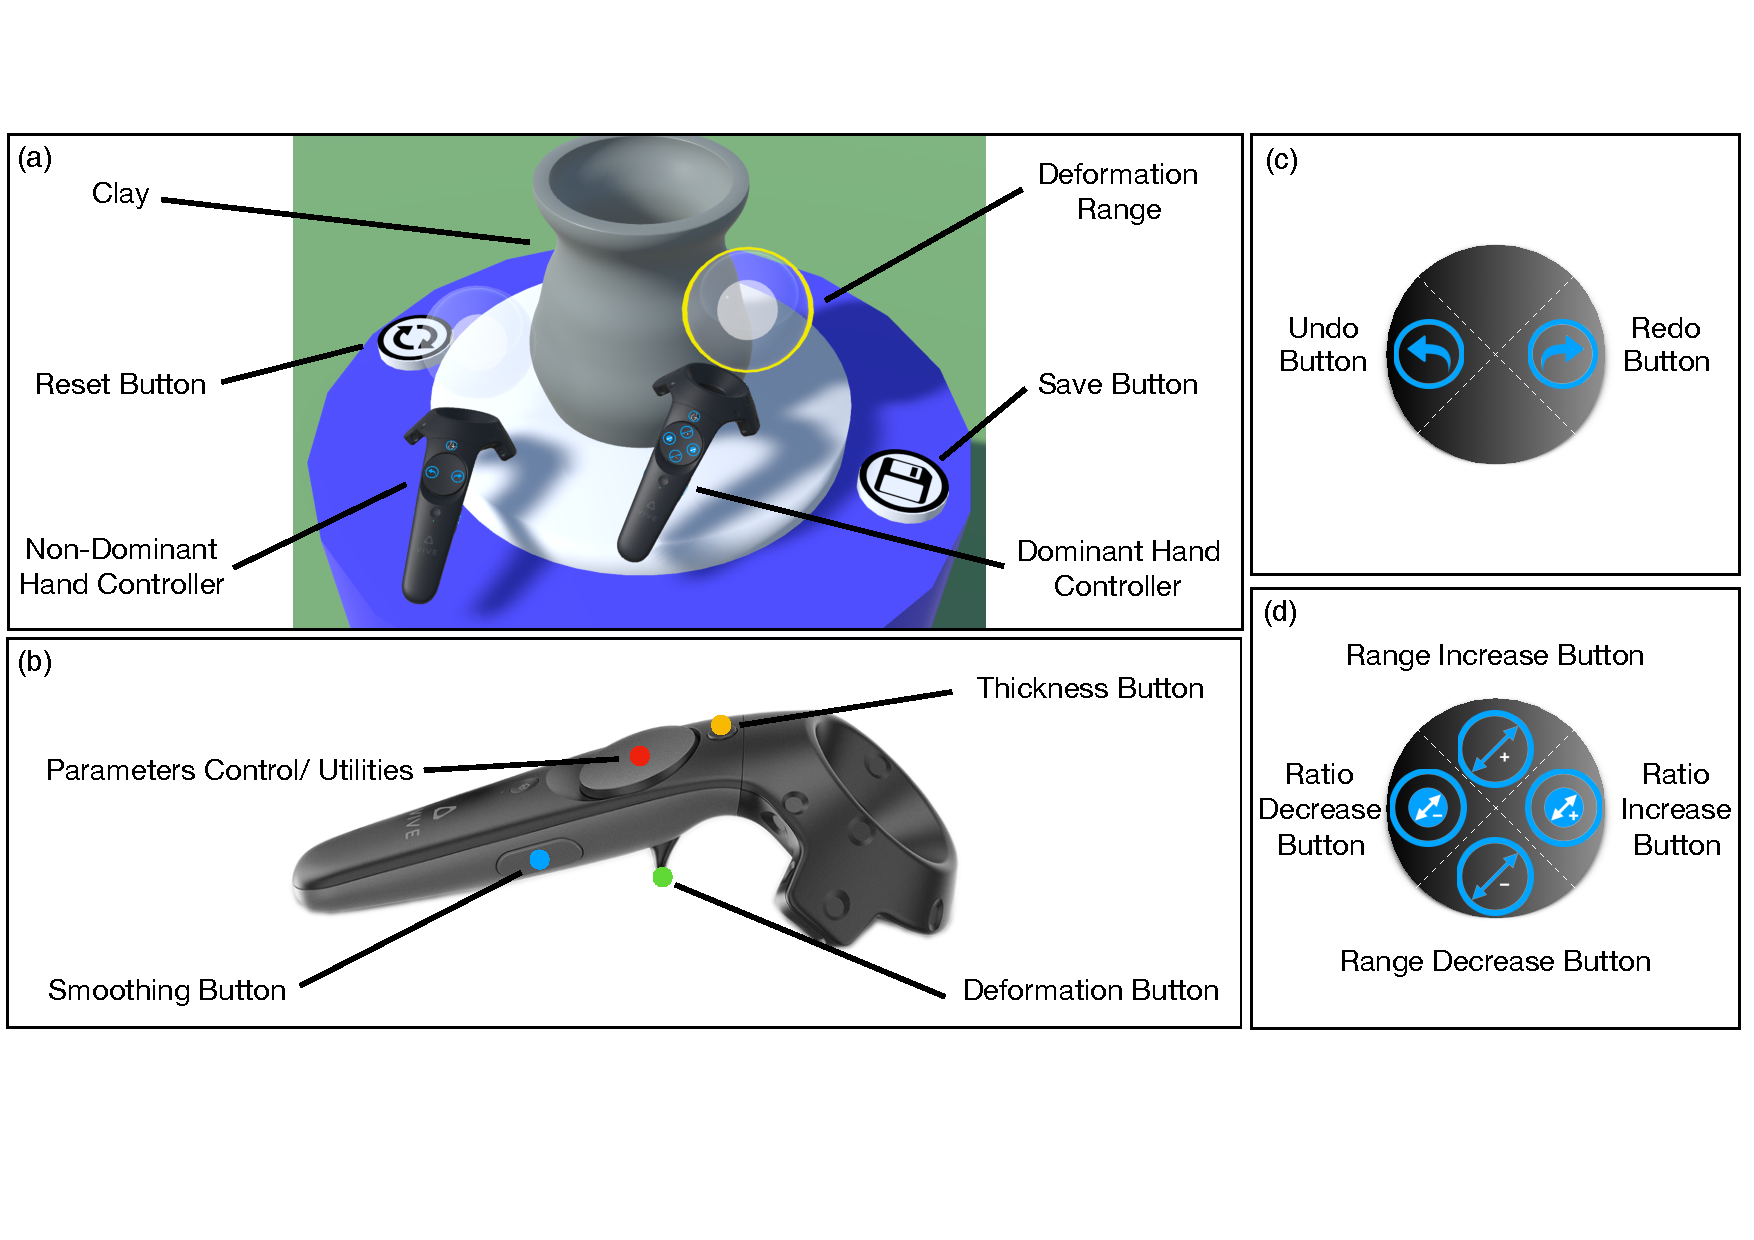
\includegraphics[width=\textwidth]{fig9}
\caption{The user interface of our system. (a) The pottery wheel in the virtual space. (b) The controller button configuration of RealPot. (c) The button layout of left controller pad. (d) The button layout of right controller pad.}
\label{fig:ui}
\end{figure*}


\subsection{System Configurations}
\label{sec:config}

%platform
We have implemented RealPot using Unity3D \cite{website:unity} game engine. RealPot is built on a HTC Vive VR system with a PC (2.10 GHz Dual Core CPU, 16 GB RAM and NVIDIA GeForce GTX 1080 graphics card) running 64-bit Windows 10 Professional.

In order to get performance statistics of the mesh generator, RealPot is tested to generate 4 models with different resolutions.
Based on the common size of clay placed on pottery wheels, we set the height 0.2 units with the radius 0.15 units.
The outer range of the handles is set to 0.2 units, and the inner range is set to 0 to get smooth deformation effect as the process begins. The centering parameter $\lambda$, height parameter $\gamma$ and smoothing parameter $\omega$ are set to 0.5, 0.4 and 0.7 respectively, in order to get a more realistic deformation via damping. The parameters for Perlin noise generation are listed in Table \ref{tab:1}. These parameters are fine tuned to get a realistic look of the clay.
%tables
Table \ref{tab:2} demonstrates statistics based on different mesh solutions. Higher resolution requires more generation time, since more vertices and triangles need to be calculated and assigned. In general, the performance of mesh generator is sufficient for the requirement in RealPot.

%[noise parameters]
% For tables use
\begin{table}
% table caption is above the table
\caption{The random parameters based on Perlin Noise.}
\label{tab:1}       % Give a unique label
% For LaTeX tables use
\begin{tabular}{lll}
\hline\noalign{\smallskip}
Parameter Name & Value & Meaning  \\
\noalign{\smallskip}\hline\noalign{\smallskip}
$a_{c}$ & 0.40 & Center Noise Amplitude \\
$a_{r}$ & 0.29 & Row Noise Amplitude \\
$a_{i}$ & 0.18 & Individual Noise Amplitude \\
$b_{c}$ & 0.81 & Center Noise Span \\
$b_{r}$ & 3.19 & Row Noise Span \\
$b_{i}$ & 0.86 & Individual Noise Span \\
$b_{a}$ & 3.75 & Angle Noise Span \\
\noalign{\smallskip}\hline
\end{tabular}
\end{table}

\begin{table}
% table caption is above the table
\caption{Statistics for different axis and height segments.}
\label{tab:2}       % Give a unique label
% For LaTeX tables use
\begin{tabular}{lllll}
\hline\noalign{\smallskip}
Axis Segments & Height Segments & Vertices & Triangles & Generation Time (ms)\\
\noalign{\smallskip}\hline\noalign{\smallskip}
60 & 100 & 12242 & 24120 & 21.48 \\
60 & 200 & 24242 & 48120 & 41.53 \\
120 & 100 & 24482 & 48240 & 42.02 \\
120 & 200 & 48482 & 96240 & 101.00 \\
\noalign{\smallskip}\hline
\end{tabular}
\end{table}

%%%Fig%%% pots
\begin{figure*}
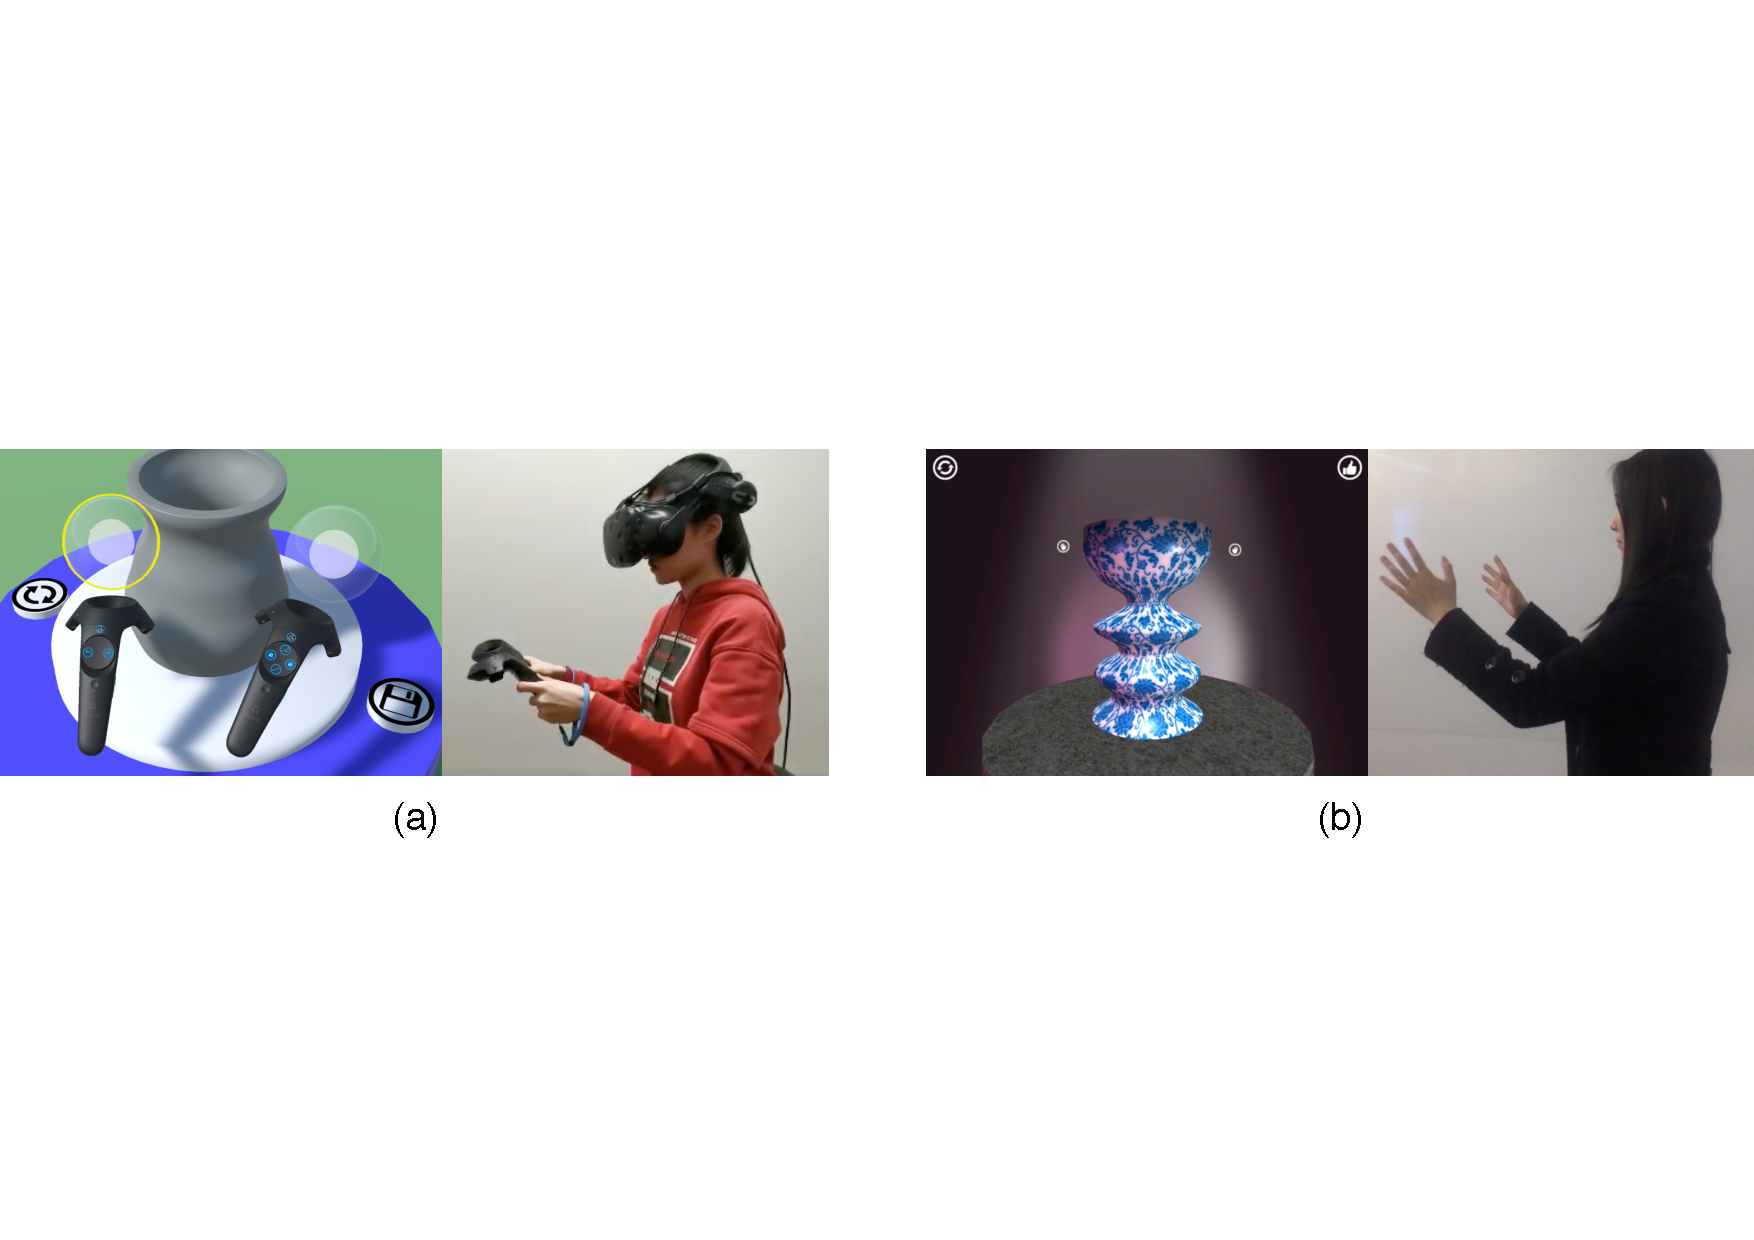
\includegraphics[width=\textwidth]{fig13}
\caption{The virtual pots designed by our system, which are real-time rendered in Unity3D.}
\label{fig:pots}
\end{figure*}

\section{User Study}
\label{sec:study}

The goal of our user study was to evaluate ...

//key

the order of ... was counterbalanced between subjects.

evaluate the components of A and B while controlling other components

//tasks


//participants


//metrics
objective user performance and subjective judgments of usability

For user performance, we measured completion time and accuracy.

For usability and preferences, we developed our own usability questionnaire consiting of seven-point Likert-scale items (See Appendix A)


//procedure
1. Each participant was required to fill out a background survey, which collected general demographic information and experiences of VR, real pottery and 3D modeling tools.

2. In the next phase, each participant experience a quick VR training for five minutes.
Since it is possible that the participants are first time users to virtual reality, that subjective may be influenced by 
Hence, we hoped VR familiarity could eliminate "wow-factor" situations.



\subsection{User Study 1: Haptic Models Comparision}
\label{sec:study1}

\subsubsection{Evaluated System}

// In user study 1, we investigated how different haptic models can influence usability.


\subsubsection{Participants}
// paticipants
19 participants were participated in our user study, 10 males and 9 females, whose age ranged from 8 to 32 years. 8 of the subjects are familiar with VR systems (42.1\%); 2 of the subjects have experience with 3D modeling tools (10.5\%); 4 of the subjects have amateur pottery throwing experience in real life (21.1\%).


\subsubsection{Experimental Design and Procedure}


// tasks


// In the case without haptic model, RealPot did not provide any haptic feedback, even if the cursor touches the virtual clay.

// In the case with the basic haptic model, the system provided haptic feedback that change according to the amount that user pulled the trigger on the handheld controller.


// each participant evaluated the basic and advanced model using a seven-point Likert scale, with 1 being the most negative score, 7 the most positive and 4 the baseline with no haptic model.

// The order of the three different conditions (i.e. no haptic model, basic haptic model and advanced haptic model) and the five tasks was assigned at random for each participant.





\subsubsection{Study Results}

// The results show that ... FIG

// All participants commented that

// more comments from individuals


// From these results, the effectiveness of the mechanism in RealPot has been demostrated.

\begin{figure*}
	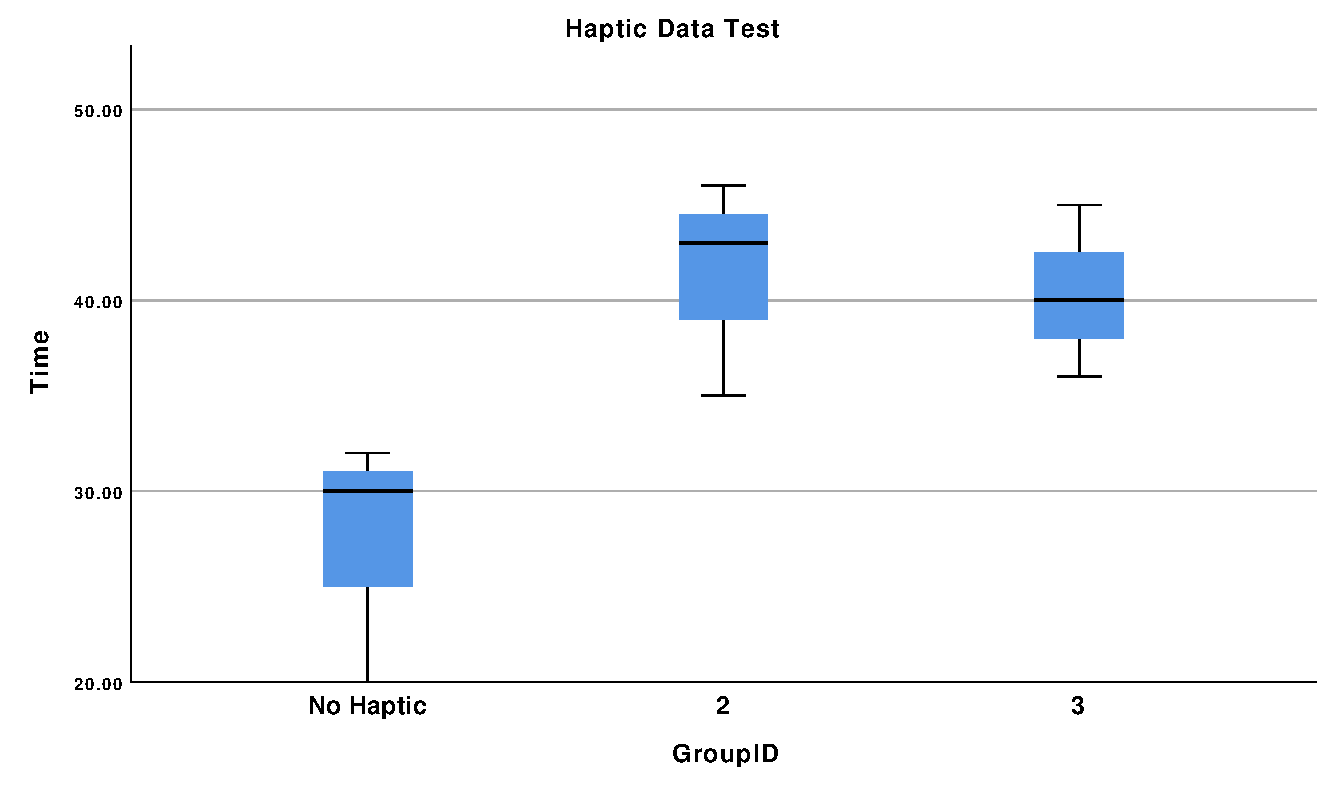
\includegraphics[width=\textwidth]{haptic_time.pdf}
	\caption{user study 1 result here}
	\label{fig:u1r}
\end{figure*}

\begin{table}
% table caption is above the table
\caption{User study 1 stats}
\label{tab:u1}       % Give a unique label
% For LaTeX tables use
\begin{tabular}{lllll}
\hline\noalign{\smallskip}
Axis Segments & Height Segments & Vertices & Triangles & Generation Time (ms)\\
\noalign{\smallskip}\hline\noalign{\smallskip}
60 & 100 & 12242 & 24120 & 21.48 \\
60 & 200 & 24242 & 48120 & 41.53 \\
\noalign{\smallskip}\hline
\end{tabular}
\end{table}

%%%


//In order to compare our system with prior CAD systems that can design virtual pottery on desktop and tablet platforms, we set up a comparative user study. We chose Autodesk Maya \cite{website:maya} as a representative of desktop modeling systems and Let's Create! Pottery (LCP) \cite{website:letspottery} as a representative of tablet pottery design systems.

\subsection{User Study 2: vs other vp}
\label{sec:study2}



\subsubsection{Evaluated Systems}

In user study 2, we investigated how our system compared with other virtual pottery systems.

// since these systems are hard to obtain, we use DigiClay as a representative bare-hand based pottery system.

// features in DigiClay

DigiClay is a virtual pottery system based on depth camera, with which the user can create pottery works using bare hands. //FIG

The interface 

The comparison is listed in the table.


\begin{figure*}
	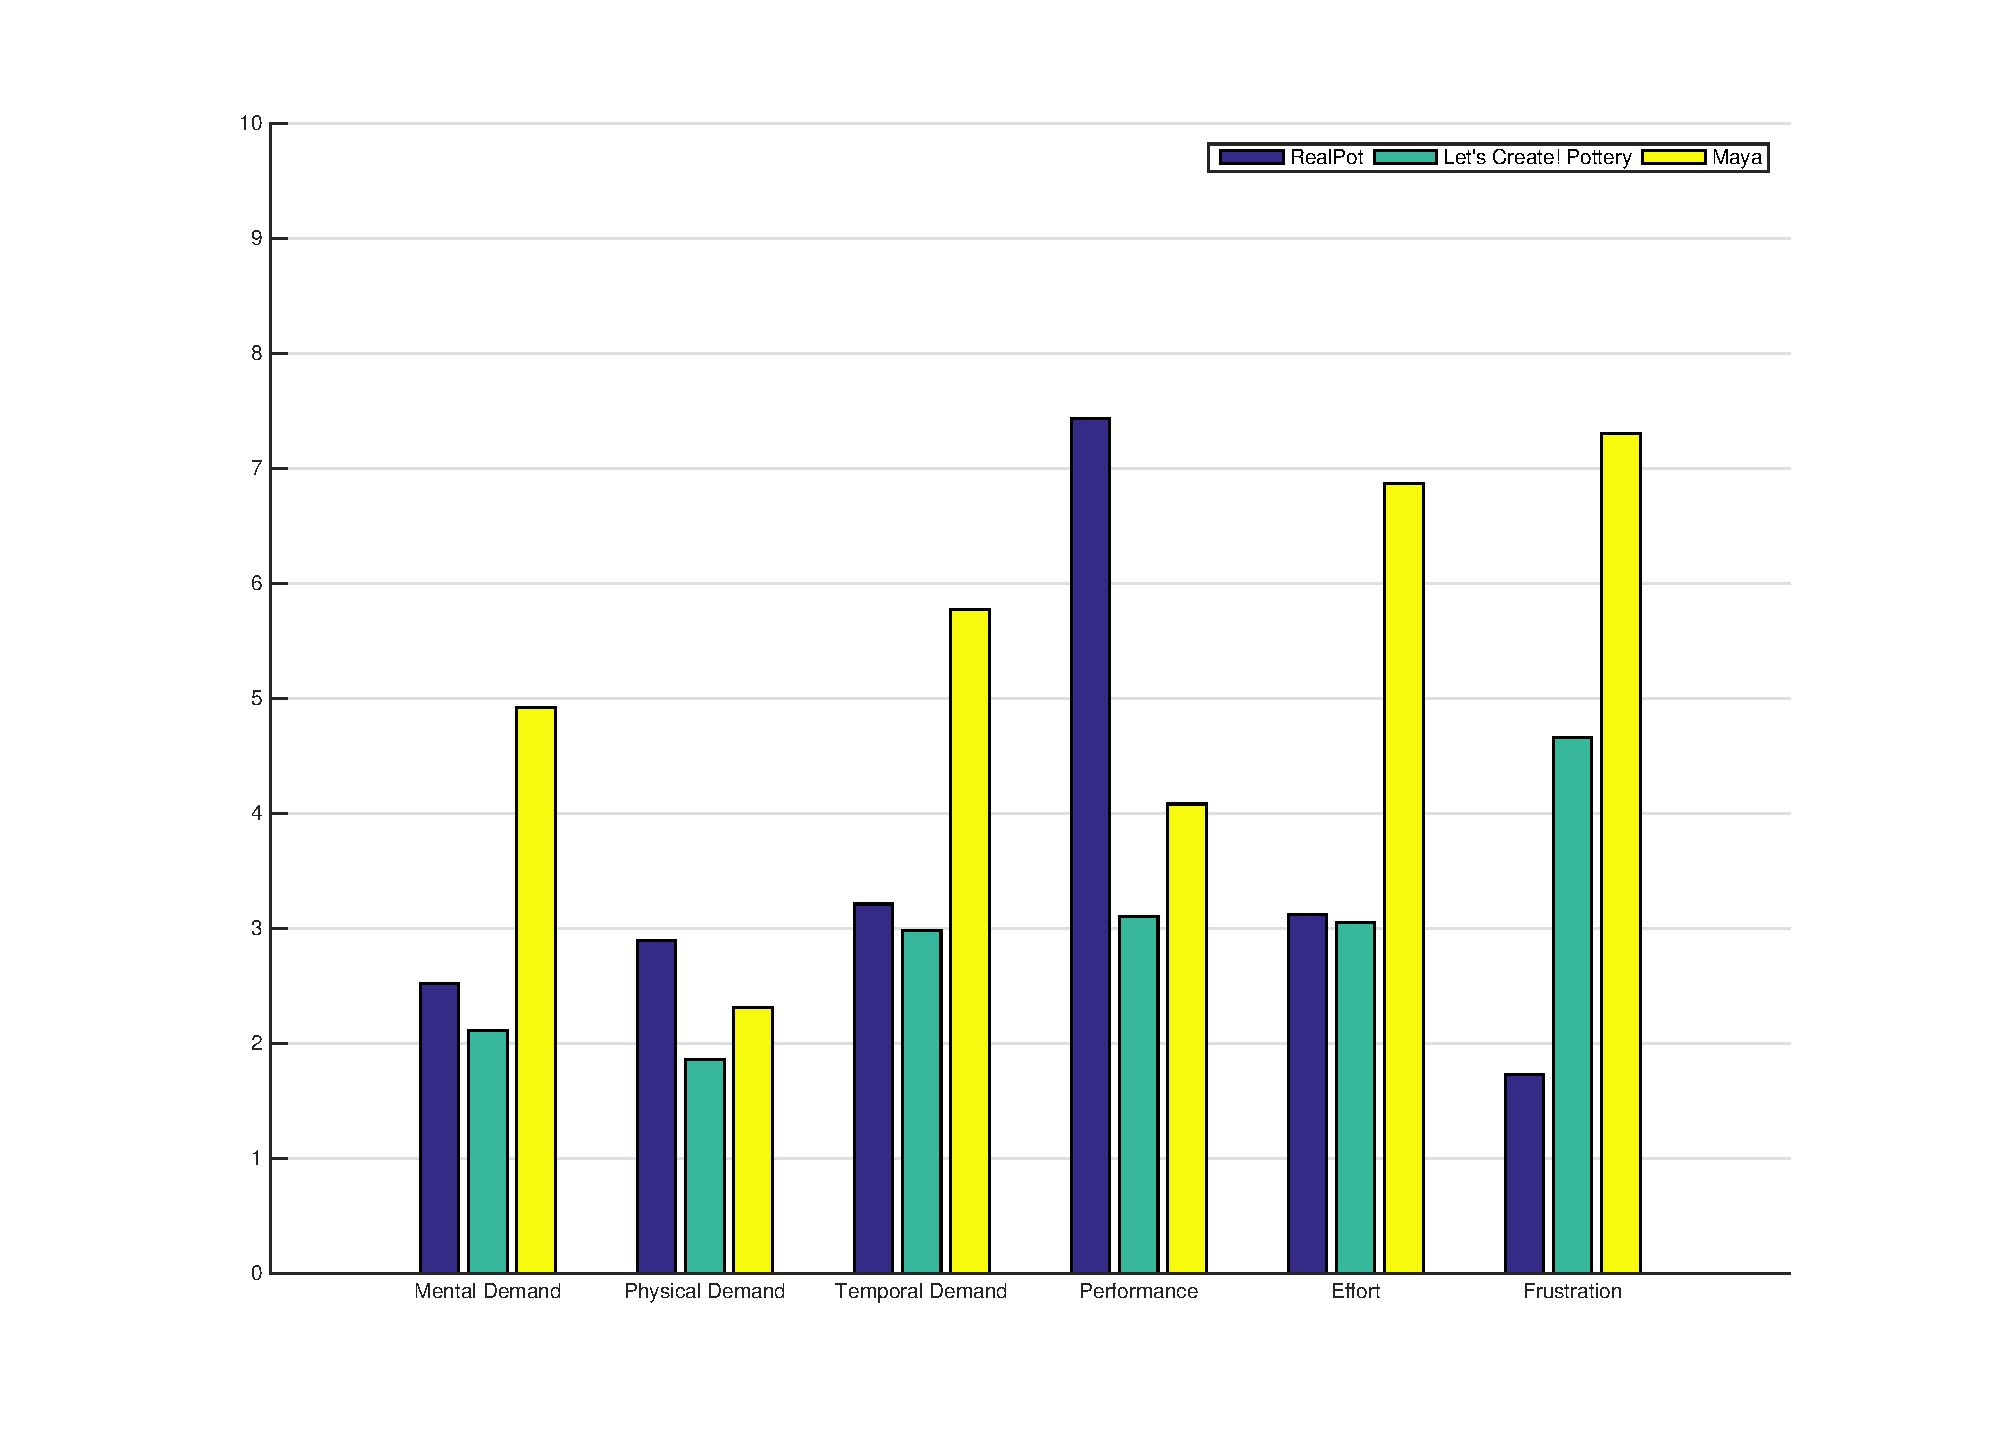
\includegraphics[width=\textwidth]{fig14.eps}
	\caption{DigiClay here}
	\label{fig:dc}
\end{figure*}

//TABLE

\begin{table}
% table caption is above the table
\caption{A comparison of two virtual pottery systems used in our user study.}
\label{tab:3}       % Give a unique label
% For LaTeX tables use
\begin{tabular}{llll}
\hline\noalign{\smallskip}
System & Input Device & Immersion & Haptic Feedback \\
\noalign{\smallskip}\hline\noalign{\smallskip}
RealPot & Hand-held Controllers & Yes & Yes \\
DigiClay & Depth Camera & No & No \\
\noalign{\smallskip}\hline
\end{tabular}
\end{table}


\subsubsection{Participants}

//participants

19 participants were participated in our user study, 10 males and 9 females, whose age ranged from 8 to 32 years. 8 of the subjects are familiar with VR systems (42.1\%); 2 of the subjects have experience with 3D modeling tools (10.5\%); 4 of the subjects have amateur pottery throwing experience in real life (21.1\%).


\subsubsection{Experimental Design and Procedure}

//tasks


Speed and accuracy are the most impoartant task performance metrics.

However, due to the implicit relationship between speed and accuracy, one can go faster but be less accurate, or can increase accuracy by decreasing speed.

it is impossible to do a task as quickly and precisely as possible.

// Accuracy first

//evaluation method (time, accuracy)



\subsubsection{Study Results}


// The results show that ... FIG

// All participants commented that

// more comments from individuals

//FIG

\begin{figure*}
	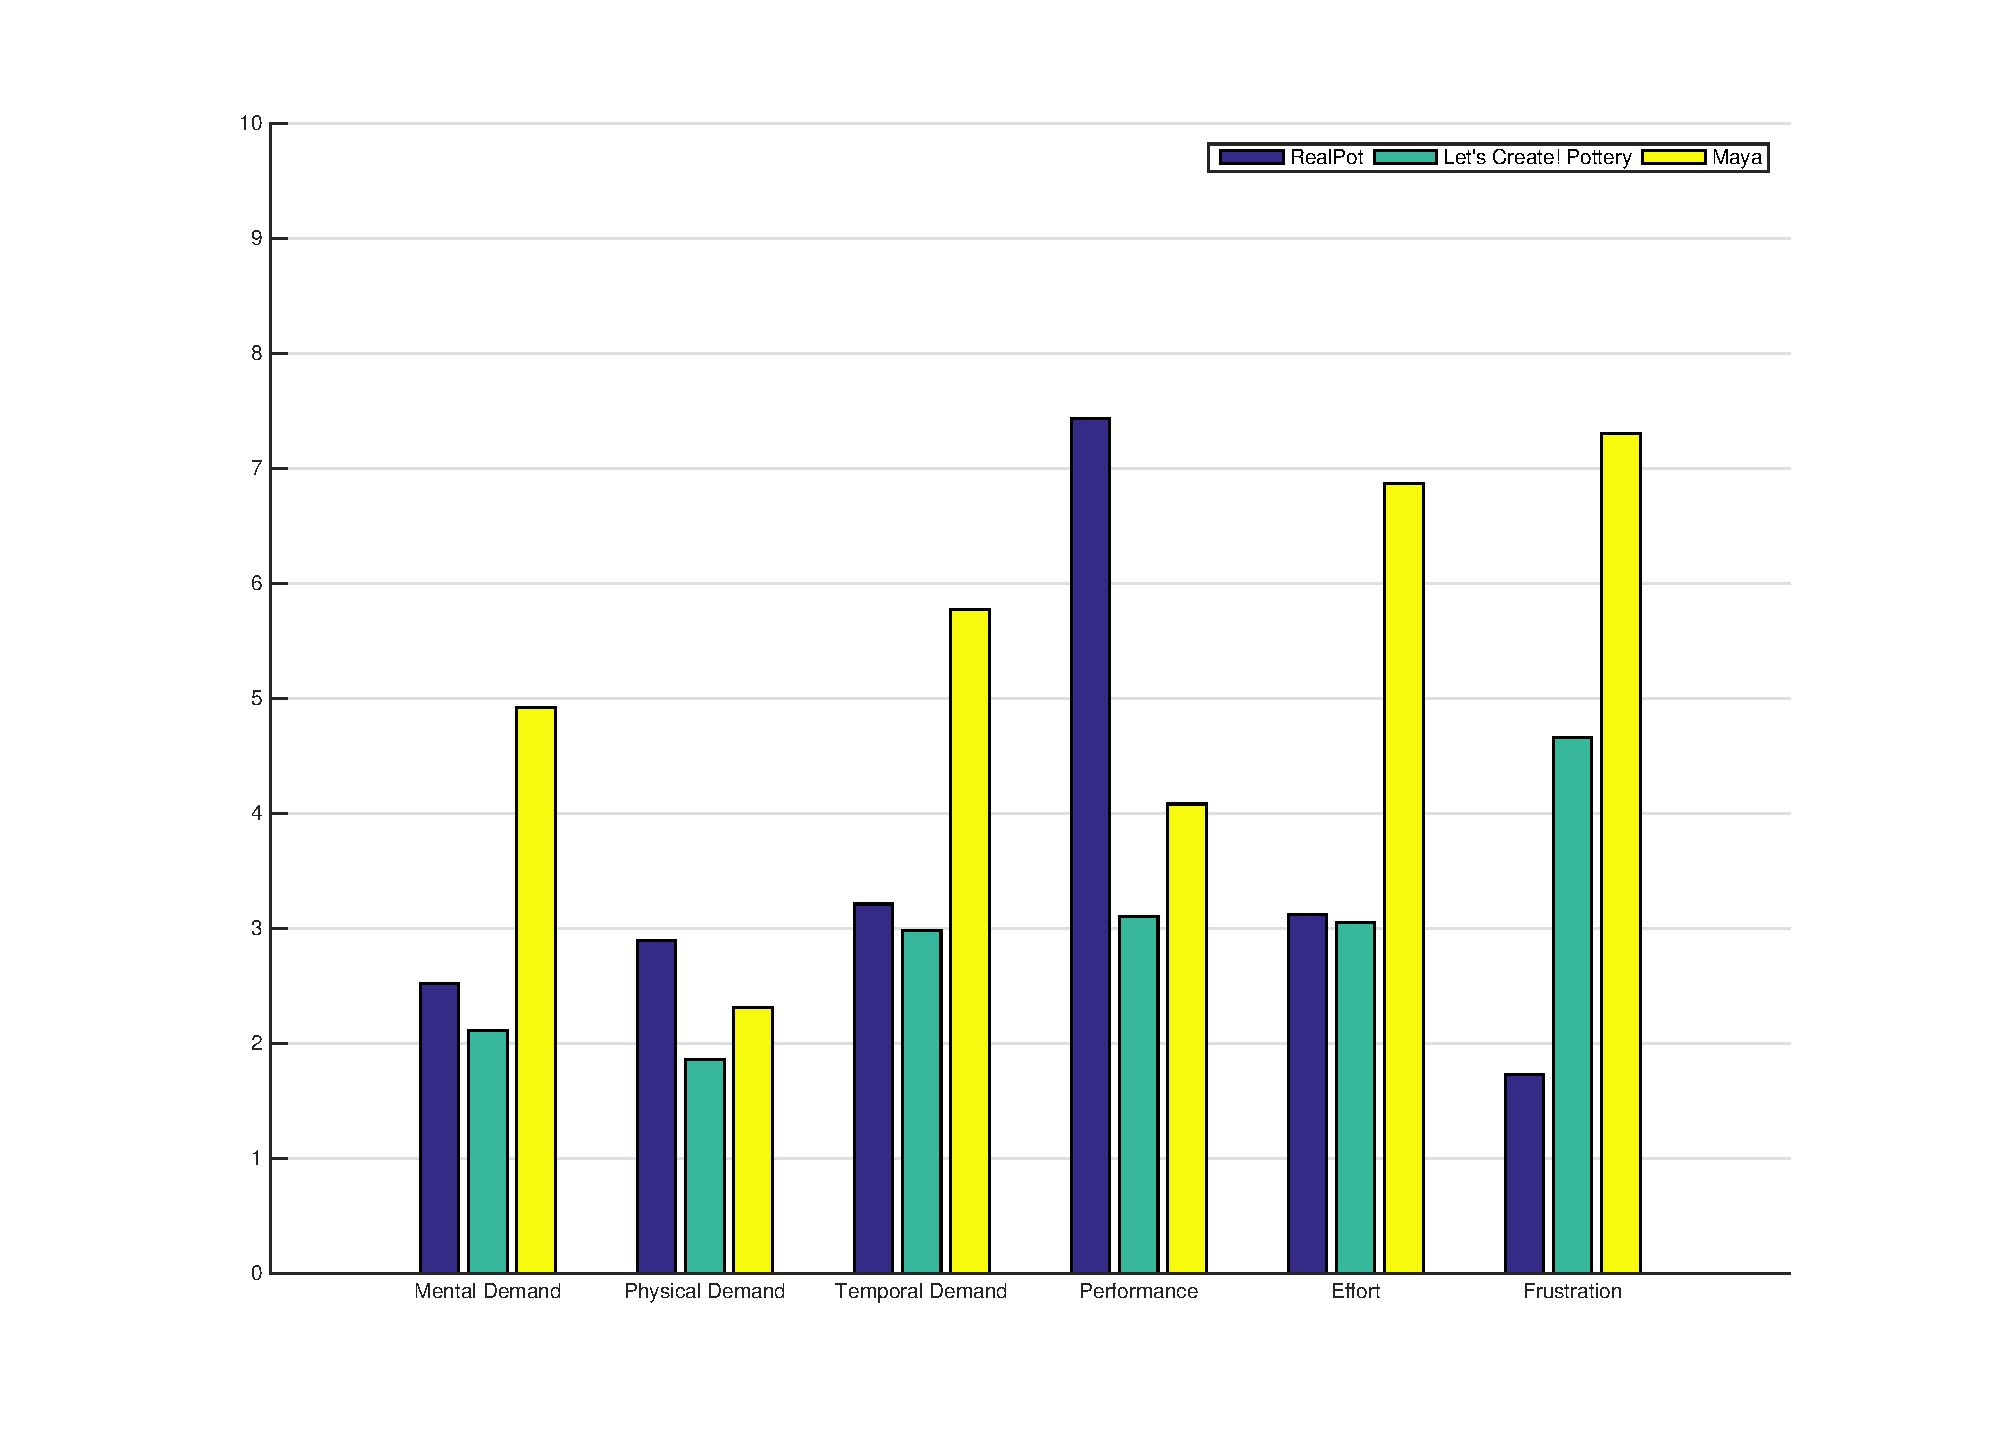
\includegraphics[width=\textwidth]{fig14.eps}
	\caption{user study 2 result here}
	\label{fig:u2r}
\end{figure*}


// From these results, the effectiveness of RealPot has been demostrated.


%%%%%%%%%%%%%%%%%%%%%%%%%%%%%%%%%%%%%%%%%%%%%%%%%%%%%%%
///////////////////////////////////////////////////////


\subsection{User Study 3: RealPot vs other cad system}
\label{sec:study3}
%GOAL
%RealPot vs Maya
To investigate the influence of modeling pipeline, we compare RealPot and Autodesk Maya since they both support 3D modeling. They differ in workflow to create and edit meshes. While RealPot can automatically generate a mesh for deformation with motion controllers, Maya needs to create a mesh from a primitive cylinder in order to edit in vertex mode, edge mode or face mode with mouse and keyboard. 
%RealPot vs Lets
On the other hand, RealPot and LCP have similarities in their workflows with intuitive interactions. They both allow users deform the mesh interactively with natural user interfaces. While RealPot enables parameter control and spatial interaction, LCP has no parameter control and provides touchscreen-based experience.

\subsubsection{Evaluated Systems}

The three evaluated systems were as follows:

\paragraph{RealPot}: Our virtual pottery tool based on HTC Vive VR system. The user can shape the virtual clay with bimanual spatial interactions.
\paragraph{Let’s Create! Pottery}: A touchscreen-based pottery creation tool on mobile devices. Users can interactively create pottery models by finger swiping on the screen.
\paragraph{Autodesk Maya}: A traditional desktop 3D modeling system, which provides a set of powerful tools for professional 3D artists. The user can edit vertex, edge, face etc. with mouse and keyboard.

The interfaces of all the three systems are demonstrated in Figure \ref{fig:sys}, and a comparison of interactions in these systems is listed in Table \ref{tab:3}. 
Although the three systems are different, we focus on comparing them based on their similarities and workflows.

%%%Fig%%% Sys
\begin{figure*}
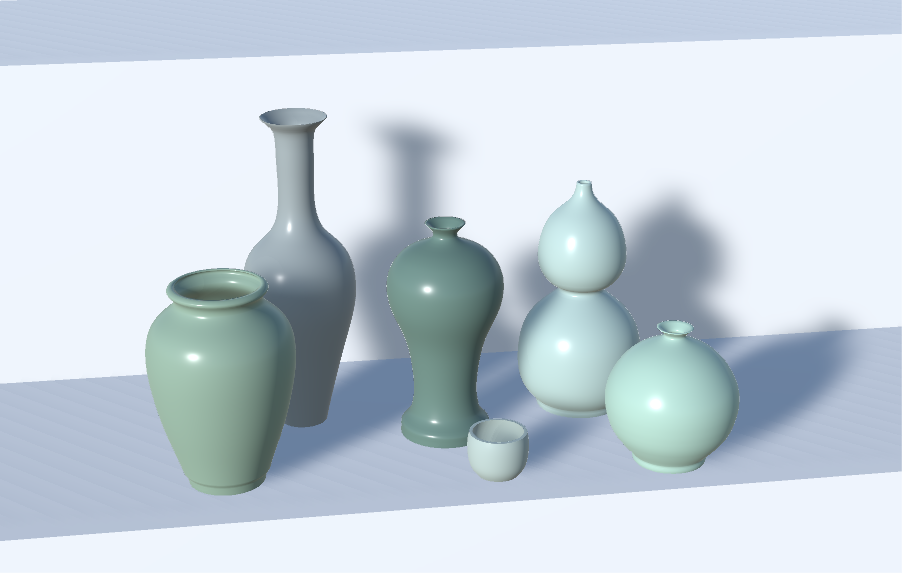
\includegraphics[width=\textwidth]{fig11}
\caption{The three systems used in our user study. (a) A virtual reality system RealPot proposed by us. (b) A touchscreen-based system Let's Create! Pottery. (c) A desktop modeling tool Autodesk Maya.}
\label{fig:sys}
\end{figure*}

% For tables use
\begin{table}
% table caption is above the table
\caption{A comparison of interactions in the three systems used in our user study.}
\label{tab:33}       % Give a unique label
% For LaTeX tables use
\begin{tabular}{llllll}
\hline\noalign{\smallskip}
System & Platform & Input Method & Head Tracking & Stereoscopy & 2D or 3D UI \\
\noalign{\smallskip}\hline\noalign{\smallskip}
RealPot & PC & Hand-held Motion Controllers & Yes & Yes & 3D \\
LCP & iPad & Touchscreen & No & No & 2D \\
Maya & PC & Keyboard and Mouse & No & No & 2D \\
\noalign{\smallskip}\hline
\end{tabular}
\end{table}

\subsubsection{Participants}
19 participants were participated in our user study, 10 males and 9 females, whose age ranged from 8 to 32 years. 8 of the subjects are familiar with VR systems (42.1\%); 2 of the subjects have experience with 3D modeling tools (10.5\%); 4 of the subjects have amateur pottery throwing experience in real life (21.1\%).
%Figure \ref{fig:11} shows two subjects using our system to throw pottery. Figure \ref{fig:12} shows more results created by the subjects.

\subsubsection{Experimental Design and Procedure}

%%%Fig%%%
\begin{figure*}
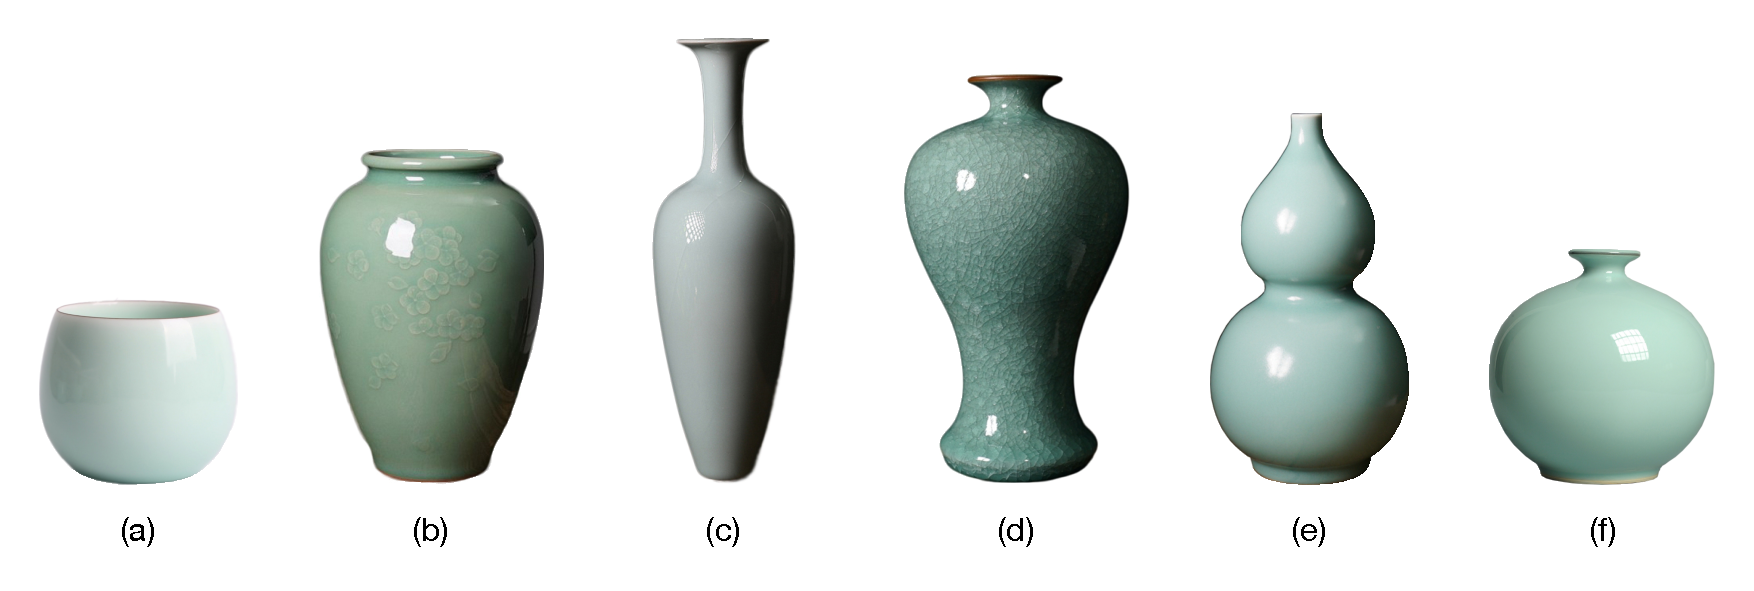
\includegraphics[width=\textwidth]{fig12}
\caption{The target shapes used in our user study, which have various heights and curvatures.}
\label{fig:target}
\end{figure*}

\paragraph{Practice} Each subject was given 15 minutes to get familiar with these systems (5 minutes for each). Subjects can ask questions whenever they need help.

\paragraph{Task 1} After the 15-minute practice of the three systems, each subject need to accomplish 3 tasks:

\textbf{T}\textsubscript{1}: Given a sequence of reference pot models as target shapes, the subjects were asked to create same pots from irregular generated meshes using RealPot. 

\textbf{T}\textsubscript{2}: Given reference pot models of the same order in \textbf{T}\textsubscript{1}, the subjects need to model these pots using Let's Create! Pottery on an iPad Pro.

\textbf{T}\textsubscript{3}: Given reference pot models of the same order in \textbf{T}\textsubscript{1} and \textbf{T}\textsubscript{2}, the subjects need to model these pots using Maya on a PC.

%[Task details]
When doing tasks \textbf{T}\textsubscript{1} to \textbf{T}\textsubscript{3}, a total of six target shapes were presented to subjects in a randomized sequence (Figure \ref{fig:pots}).
%%% TODO

%[NASA-TLX]
\paragraph{Questionnaire 1} After accomplishing each task, the subjects were asked to answer a questionnaire with six questions to measure the six dimensions of NASA-TLX, which includes physical demand, mental demand, temporal demand, effort, performance and frustration. 5 additional questions were asked after they finished all tasks.

%[Some explanations]
NASA-TLX has been chosen in our research because it is widely used in human factor studies which addressed questions about interface design and evaluation \cite{hart2006nasa}.
We selected NASA-TLX as a part of our questionnaire to assess user workload in the three systems.
Since the functionalities are different among the three systems, it is impossible and unfair to compare the interactions.
We intended to allow our subjects to experience those differences and similarities through these tasks and analyze which types of interactions and results were more attractive to them through our user study questions.

\paragraph{Task 2} After finishing tasks \textbf{T}\textsubscript{1} to \textbf{T}\textsubscript{3}, each subject need to accomplish 3 more tasks:

\textbf{T}\textsubscript{4}: Use RealPot to make a creative pottery model freely.

\textbf{T}\textsubscript{5}: Use Let's Create! Pottery to make a creative pottery model freely.

\textbf{T}\textsubscript{6}: Use Maya to make a creative pottery model freely.

\paragraph{Questionnaire 2} Each subject needs to answer the following questions after finishing tasks \textbf{T}\textsubscript{4} to \textbf{T}\textsubscript{6}:

\textbf{Q}\textsubscript{1}: Rank the three systems according to ease of learning from high to low.

\textbf{Q}\textsubscript{2}: Rank the three systems according to their supports for your imagination and creativity from high to low.

\textbf{Q}\textsubscript{3}: Rank the three systems according to your preference from high to low.


\subsubsection{Study Results}


%[basic introduction]
%Figure \ref{fig:boxplot} shows the boxplots of completion time and correlation coefficient for each target shape created in \textbf{T}\textsubscript{1}.
Figure \ref{fig:tlx} shows mean values of the six dimensions of NASA-TLX for \textbf{T}\textsubscript{1}, \textbf{T}\textsubscript{2} and \textbf{T}\textsubscript{3}.
Figure \ref{fig:ranking} shows the vote results of \textbf{Q}\textsubscript{1}, \textbf{Q}\textsubscript{2} and \textbf{Q}\textsubscript{3}, where we count a score of 3 for the system in the highest ranking and 1 for the system in the lowest ranking. 

%%%Fig%%% tlx
\begin{figure*}
	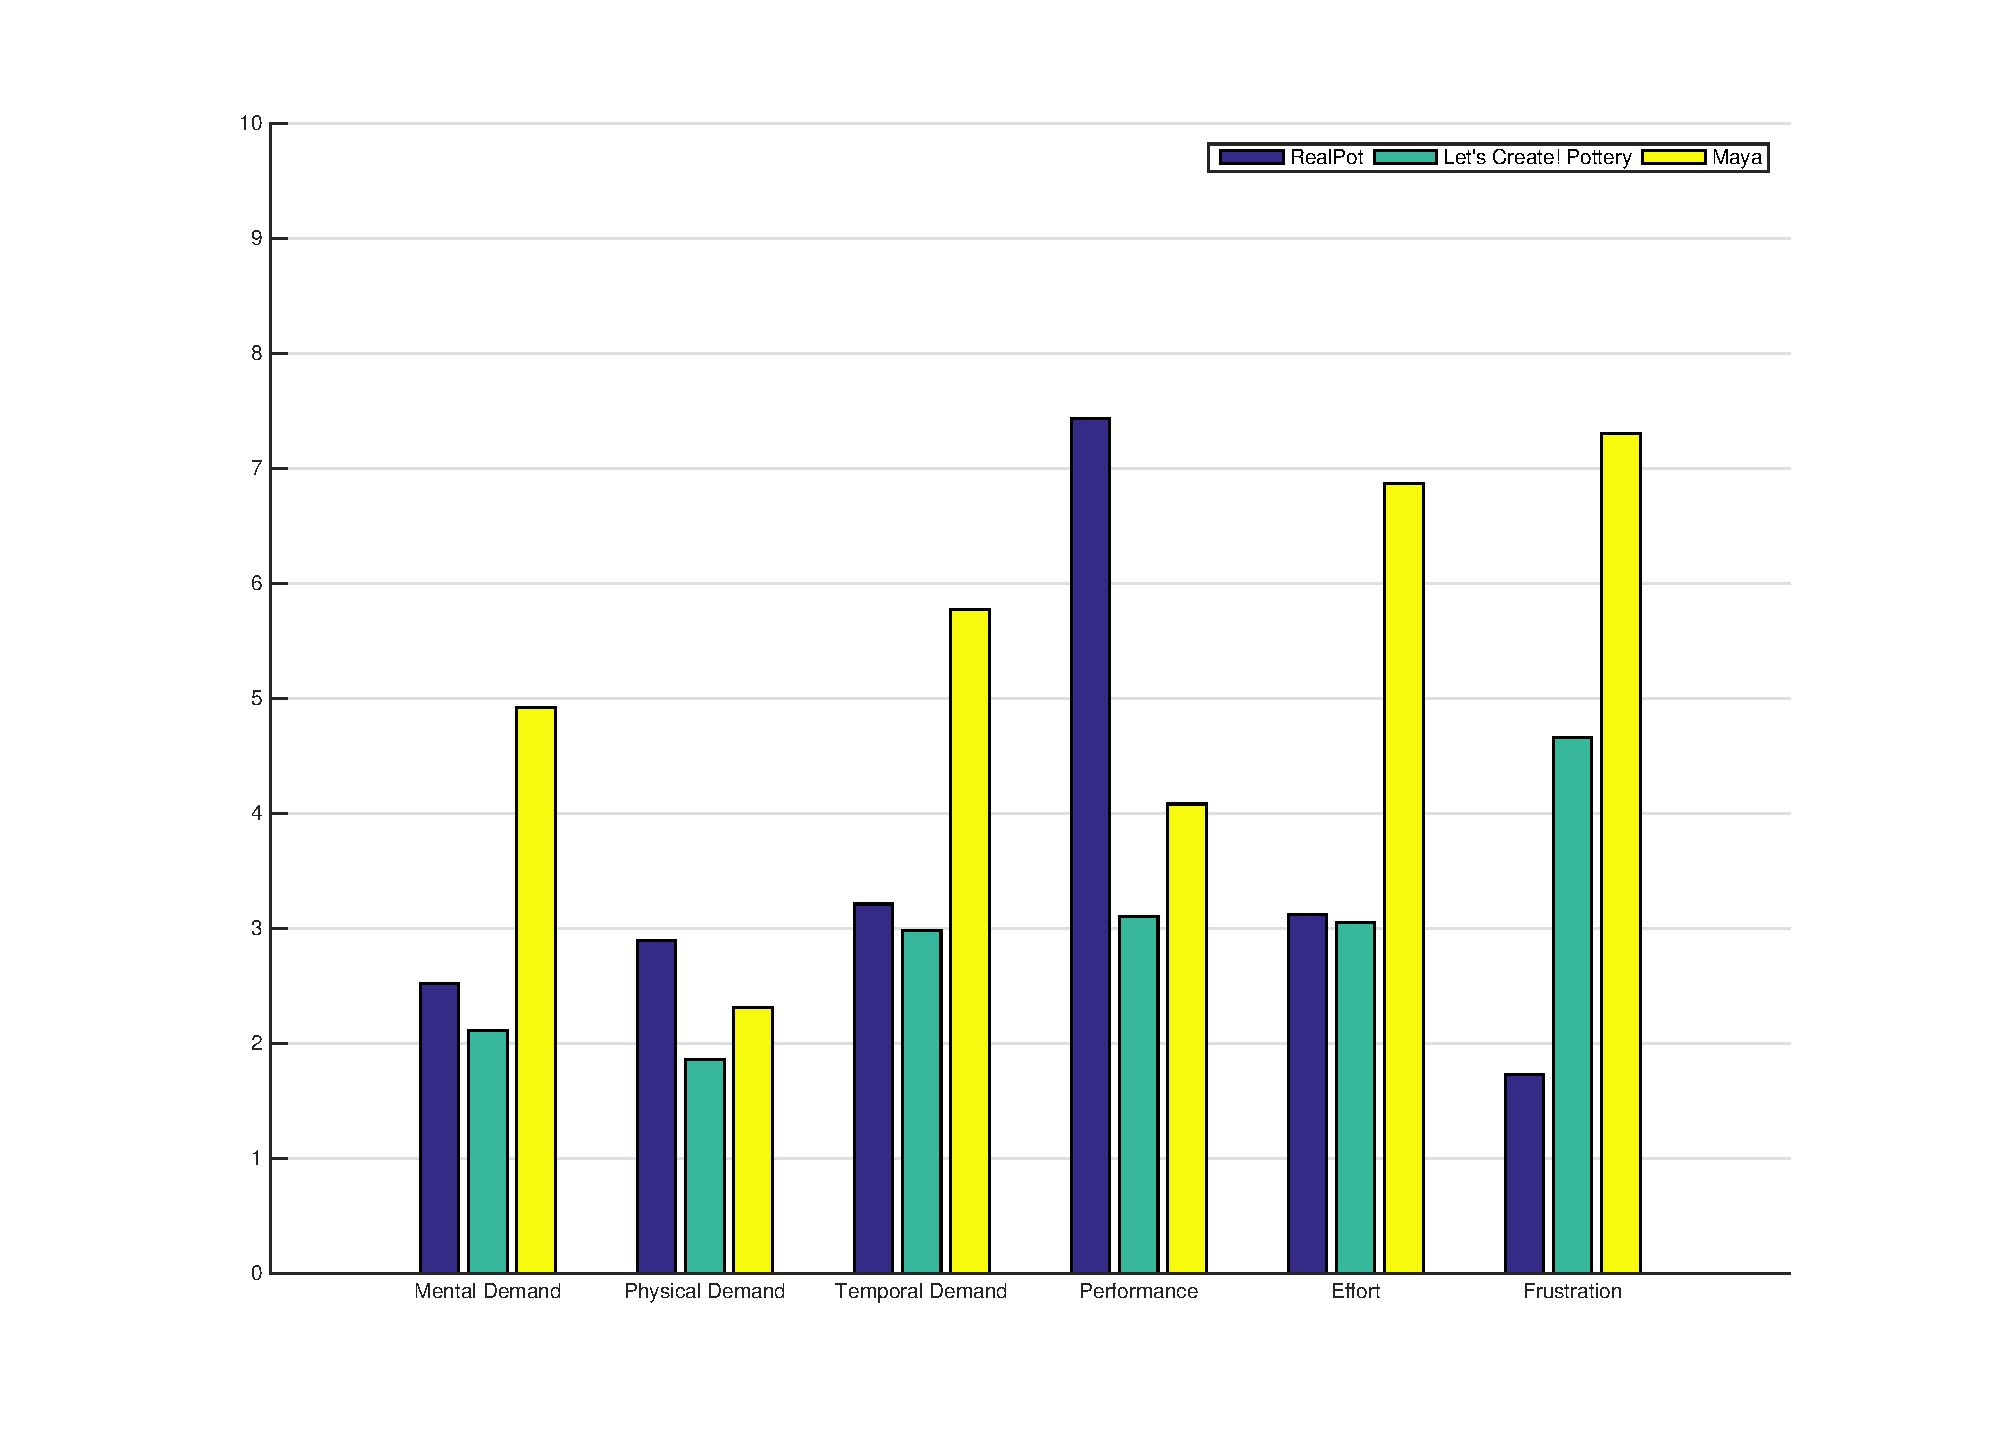
\includegraphics[width=\textwidth]{fig14.eps}
	\caption{Mean values of the six dimensions of NASA-TLX.}
	\label{fig:tlx}
\end{figure*}

%mental/physical/temporal
According to Figure \ref{fig:tlx}, we can get some findings. 
Firstly, the mental demand values of \textbf{T}\textsubscript{1} (M = 2.52) and \textbf{T}\textsubscript{2} (M = 2.11) were almost the same and much lower than the value of \textbf{T}\textsubscript{3} (M = 4.92). Similarly, the temporal demand value of \textbf{T}\textsubscript{3} (M = 5.77) was much higher than the values of \textbf{T}\textsubscript{1} (M = 3.21) and \textbf{T}\textsubscript{2} (M = 2.98). This indicated that RealPot and LCP were easier to use and less time-consuming than Maya. Unsurprisingly, the physical demand value of \textbf{T}\textsubscript{1} (M = 2.89) is slightly higher than \textbf{T}\textsubscript{2} (M = 1.86) and \textbf{T}\textsubscript{3} (M = 2.31), which means interactions based spatial movements are slightly more laborious than touchscreen and keyboard/mouse interactions.

%[Maya - hard]
Maya showed much higher values in effort (M = 6.87) and frustration (M = 7.30) and lower value in performance (M = 4.08) compared with RealPot and LCP.
Since most subjects in the user study have no 3D modeling software experience, the complex user interface in Maya makes it challenging for these novice users to memorize where to find the commands they need, rendering a high effort.
Although keyboard-mouse based interaction allows precise controls with low physical demand, many subjects struggled with selecting and manipulating vertices and faces accurately, which caused high user frustration. As a result, most subjects were not satisfied with their performances in \textbf{T}\textsubscript{3}.

%[LCP - limitation] [thickness smooth sharpness]
Surprisingly, we found that it was not as satisfied as we predicted for the subjects using LCP in \textbf{T}\textsubscript{2}, where the performance value (M = 3.10) is lower than we expected. This is due to the limitations in LCP: Although the interaction in LCP is easy to learn, some high curvature features (Figure \ref{fig:target}b, \ref{fig:target}d, \ref{fig:target}e and \ref{fig:target}f) cannot be reached due to LCP has a fixed deformation range. Moreover, subjects cannot modify the thickness of pots, which is another limitation of LCP. Thus, the frustration value (M = 4.66) are high during \textbf{T}\textsubscript{2}.

%%%Fig%%% ranking
\begin{figure*}
	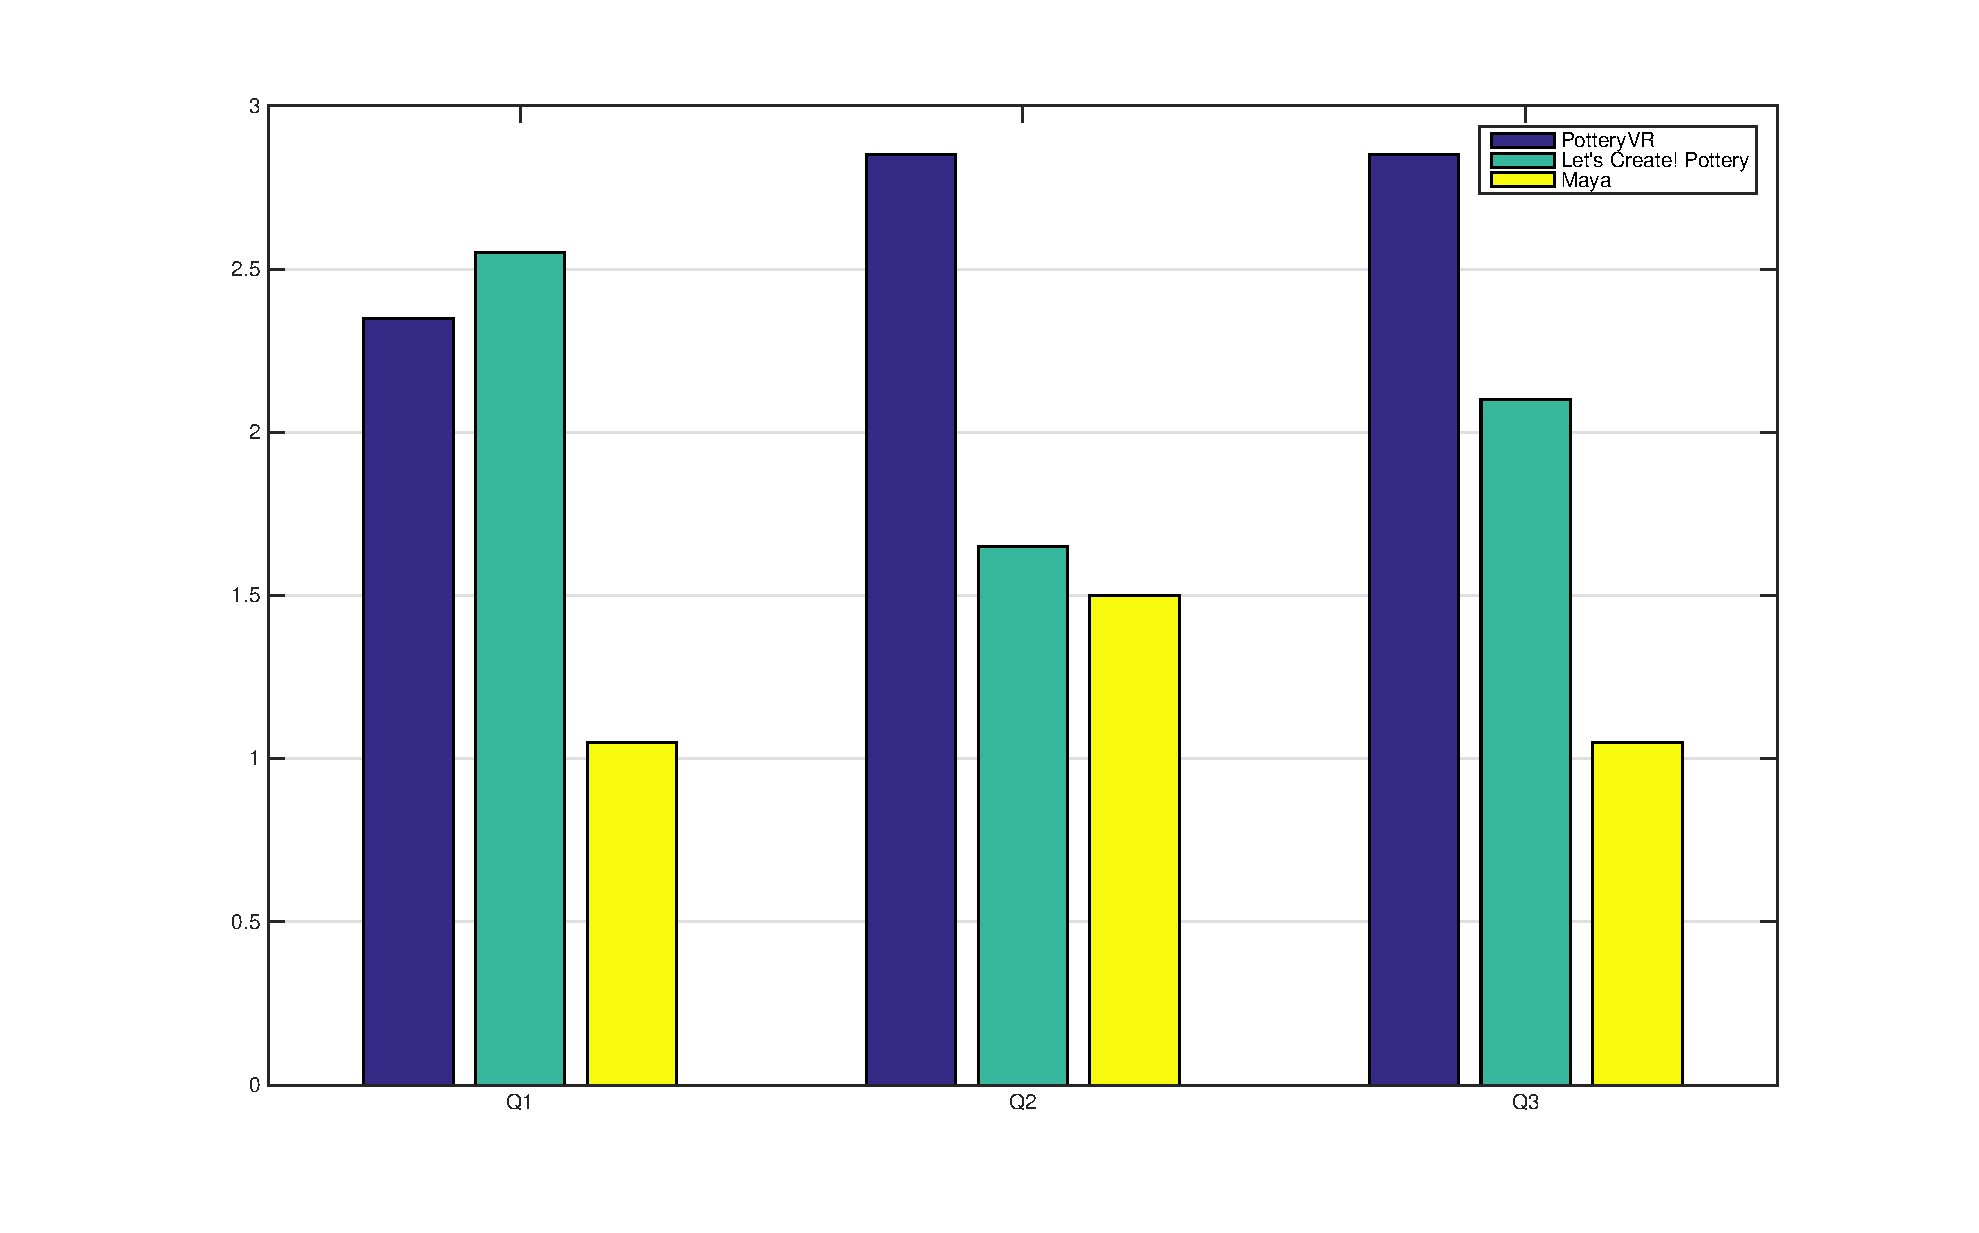
\includegraphics[width=0.75\textwidth]{fig15.eps}
	\caption{Mean ranking scores of Q1, Q2 and Q3.}
	\label{fig:ranking}
\end{figure*}

%[user preference][enjoyable and intuitive]
The voting results in Figure \ref{fig:ranking} demonstrated the ease of learning, the support of creativity and overall preference of the three systems.
%ease
Compared with the complex interfaces and the keyboard and mouse operations in Maya, RealPot and LCP provides simple interfaces and intuitive interactions, allowing users get familiar with the interaction with ease.
%creativity
In addition, most subjects considered RealPot stimulate their creativity and imagination the most. From their feedbacks, we found that spatial interactions in virtual reality context gave them a novel and realistic way to interact with virtual clay when using RealPot. Moreover, RealPot provides more powerful operations such as adjustable deformation range, thickness control and smoothing than LCP, allowing subjects creating characteristic shapes.

%overall-enjoyable, useful for training
In \textbf{Q}\textsubscript{3}, RealPot became the favorite virtual pottery system for the subjects. From user feedbacks, we found that RealPot provided the subjects with most enjoyable experience among the three systems, which also has a balance of having simple interfaces and useful functionalities. In addition, the natural bimanual interactions in RealPot are closely related to the operations in reality pottery, making it an ideal training simulation tool for pottery.


///////////////////////////////////////////////////////
%%%%%%%%%%%%%%%%%%%%%%%%%%%%%%%%%%%%%%%%%%%%%%%%%%%%%%%

\section{Results}
\label{sec:results}

For completion times, we performed a one-way ANOVA and the results showed different haptic models had a significant effect (F(1, 23) = 82.3503, p < 0.0001). 





\section{Discussions}
\label{sec:discussion}
%[Positive]
We collected user feedbacks after the subjects had used our system. In summary, subjects gave many positive feedbacks when using our system to design pottery models. They spoke highly of the immersive pottery creation experience with intuitive interactions and haptic feedbacks that motivated them to design pottery works just like working on real clay. In addition, the undo/redo functionalities are quite convenient according to the subjects, which enhances the efficiency during creation processes. For those who have no real-life pottery creation experience enjoyed our system very much and would like to try real pottery someday. 

%[Suggestions]
During our user study, we found that the undo/redo functionality is not used frequently as we expected.
The reason might be that the changes for each operation are not so difficult to revert, that some users just manually fix the change without using undo/redo shortcut provided by RealPot.

We also asked their suggestions for the future features they wanted to see in RealPot.
A few subjects expressed their wishes to add coloring feature, which allows them decorate the pots with colors and patterns.
At the end of our user study, many subjects said they would like to try RealPot one more time.

%[limitations]
Our system still has its limitations. First, the physical size of the motion controllers sometimes affect the deformation in bimanual mode, especially when the part of the clay is narrow that two controllers may collide with each other. For example, when subjects working on the neck of clay, it will be difficult to edit with two controllers. This problem can be easily solved by providing user one-hand deformation mode. We plan to use data gloves to avoid these situations in the future.
%
Second, the potteries designed by our systems lack colors and textures. Although we focus on deformation in our study, several subjects stated that they wish to paint the pottery after designing the shape of the clay. We intend to add new features related to interactive painting on 3D objects.
%
Another limitation of our system is that it cannot adding handles to the pottery. We will introduce more features that allow users to modify the topology of the mesh in order to create more personalized pottery works.


\section{Conclusions}
\label{sec:conclusion}

We present RealPot, an immersive virtual pottery system in VR.
Closely linked to pottery creation experience in real life, our system enables users to manipulate the mesh in real time with two hands, allowing them creating a variety of pottery models from realistic generated clay meshes.
As an educational tool, RealPot can help novice users and children to learn real-life pottery creation process in virtual environments, who can fabricate their works using our system with a 3D printer.
Our results have shown that RealPot has relative advantage compared with traditional desktop 3D modeling experience (Maya) and touchscreen experience (Let's Create! Pottery).
A possible extension of our system is to support interactive coloring functionalities in the future, which can enhance the artistry of user generated pottery works.

\section*{Appendix: Usability Questionnaire}

\begin{enumerate}
\item Rate how easy
\item Rate how natual
\item Rate how much fun
\item Rate how tiring
\item Rate how much skills you gain from the virtual pottery training
\end{enumerate}


\begin{acknowledgements}
This work is supported by the Natural Science Foundation of China (No.~61502118), the Natural Science Foundation of Heilongjiang Province in China (No.~F2016028 and F2016009), the Fundamental Research Fund for the Central Universities in China (No.~HEUCF180602 and HEUCFM180604) and the National Science and Technology Major Project (No.~2016ZX03001023-005).
%If you'd like to thank anyone, place your comments here
%and remove the percent signs.
\end{acknowledgements}

% BibTeX users please use one of
%\bibliographystyle{spbasic}      % basic style, author-year citations
\bibliographystyle{spmpsci}      % mathematics and physical sciences
%\bibliographystyle{spphys}       % APS-like style for physics
\bibliography{pottery}   % name your BibTeX data base

% Non-BibTeX users please use
%\begin{thebibliography}{}
%
% and use \bibitem to create references. Consult the Instructions
% for authors for reference list style.
%
%\bibitem{RefJ}
% Format for Journal Reference
%Author, Article title, Journal, Volume, page numbers (year)
% Format for books
%\bibitem{RefB
%Author, Book title, page numbers. Publisher, place (year)
% etc
%\end{thebibliography}

\end{document}
% end of file template.tex

